\setchapterpreamble[u]{\margintoc}
\chapter{Optimization of LiDAR scans}
\labch{lidar_optimization}
\label{sec:lidar_optimization}

\section*{About this chapter}

\marginnote[13.0cm]{Although this optimization provides a minimum number of optimal scan positions, these are still required to be performed by humans. Therefore, positions must be optimized but also narrowed, in order to make this task less time-consuming.}
This chapter presents a pipeline for optimizing TLS scans in indoor environments. This optimization works over the previously implemented LiDAR simulation. To solve this problem, metaheuristics such as local search (LS), tabu search and genetic algorithms (GA) operate over a set of positions, whose fitness is measured after their synthetic LiDAR point cloud. The expected outcome is a set of optimal locations that help to scan a real-world scenario by ensuring proper density, coverage, etc. In comparison with previous research, buildings are represented by 3D models, thus allowing us to account for possible improvements provided by varying the sensor height. Furthermore, previous literature has described up to four metrics, including LOA (accuracy), LOD (detail), LOO (overlap) and LOC (coverage). This work comprises the previous four metrics into three functions that reduce the number of steps in multi-objective optimization. Following the approach of this chapter, the LiDAR scans as well as part of the optimizing algorithms were developed in the GPU and multi-core CPU otherwise. Rather than selecting among different metaheuristic algorithms, these are proposed to be chained. This works especially well for narrowing the solution space. For instance, LS helps to provide a rapid improvement of initial positions, whereas GA narrows this search space by generating a solution that encodes which positions ought to be used without distorting the metrics. I.e., \textbf{which is the minimum number of points (and which points) that help to solve the scan optimizing while still guaranteeing some minimal requirements?} This problem has been previously referred to as  the NP-complete set-coverage problem \cite{li_probability_2021, mohamadi_efficient_2021, roostapour_pareto_2022} if the number of solutions, $n$ is known. It is not known in this problem, since we are able to tell how many positions we look for unless a user establishes the value of $n$.

\begin{kaobox}[frametitle=Case study of TLS optimization: Building Information Modelling]
TLS scans are a cumbersome task operated by humans by placing the LiDAR sensor on a limited number of locations that may contribute, with better or worse results, to the composite point cloud. However, even repeatability must be guaranteed in some environments. A case study where this optimization is easier to understand is on the monitoring of buildings in the construction industry. It requires periodic scans that can be saved under the widely known Building Information Modeling (BIM) \cite{macher_point_2017}. This data representation encodes the features of a building, including 3D design drawings, materials, costs and safety specifications, and provides an interface for the management of 4D applications. Together with TLS, it enables the monitoring of continuously evolving buildings to preserve cultural heritage, track its current state and maintain repair records \cite{rocha_scan--bim_2020, andriasyan_point_2020, moyano_bringing_2020, ham_phased_2020}. However, monitoring buildings over time is time-consuming, especially in dynamic environments. Also, TLS scans are given by multiple point clouds that must be later fused, and for this task, there should exist some notable overlapping among them, or be able to distinguish visible markers otherwise \cite{gollob_comparison_2020}. In this case study, the development of tools for planning TLS surveys plays a key role. 
\end{kaobox}

The main contributions of this work are a massively parallel optimization solver using smooth objective functions, instead of being ruled by thresholds, to measure the fitness of individual scans. Starting solutions are locally enhanced, rather than using large grid subdivisions with a huge memory footprint. Then, the optimal set of locations is estimated with GA, whereas the objective function used during this optimization implicitly minimizes the number of scans. The outcome of GA is further refined to guarantee the overlapping of individual scans using a Greedy approach. The input models used during the experimentation are large CAD scenarios from BIM projects authored by Autodesk Revit\textsuperscript{\textregistered}. As a result, this work is able to provide a near-optimal set of locations aimed at optimizing the monitoring of buildings. Furthermore, these optimizations are performed using LiDAR specifications that can be adjusted to those of commercial sensors. 

\section{On the optimization of TLS scans}

3D imaging technology is widespread in the construction industry for the tracking of building progress since it acquires the environment geometry in a precise and highly detailed way. Rather than collecting their geometry as polygonal meshes, these are scanned to output 3D point clouds. In this regard, TLS has been increasingly being used to collect large datasets from buildings \cite{shariq_revolutionising_2020} and cultural heritage remains \cite{banfi_integration_2019, ham_phased_2020, andriasyan_point_2020}, among others. Some of the main shortcomings of TLS technology are the occlusion and range limitations \cite{soudarissanane_optimizing_2012}. Hence, planning TLS scans may help to mitigate this by 1) minimizing the number of scans, 2) generating a point cloud with uniform density, and 3) reducing the occlusion from scene objects. All these three objectives are equally affected by the location and configuration of the scanner. Other LiDAR technologies have arisen as suitable alternatives to TLS for addressing the aforementioned drawbacks. However, these are still recent, and despite solving some of these drawbacks, others arise. For instance, LiDARs mounted on backpacks reduce the acquisition time and cover large areas \cite{rodriguez-gonzalvez_mobile_2017}, but the path should be carefully planned to avoid occlusion and guarantee coverage. Also, their density is lower \cite{bienert_comparison_2018}.

Regarding the optimization of TLS scans in buildings, this field of research is frequently referred to as Planning for Scanning (P4S). Most of the studies narrow 3D environments to 2D cross-sections, or simplify the scene primitives into others whose collisions are easier to solve, even wrapping a set of primitives (e.g., voxelizations \cite{wakisaka_optimal_2019}). Sometimes, it requires previous knowledge of the scenario, which is not assumed in this work. For instance, AABBs and Object-Oriented Bounding Boxes (OOBB) have been previously used over environments in which AABBs did not fit well to rotated, non-planar surfaces \cite{li_3d_2022}. DSMs have also been explored in 2.5D optimizations \cite{starek_viewshed_2020}. Regarding the optimization approach, most of them are based on the iterative find of the Best Next View (BNV), while others apply heuristics such as Greedy \cite{ giorgini_sensor-based_2019},  Simulated Annealing (SA) \cite{chen_indoor_2018}, GA \cite{jia_comparison_2017}, Particle Swarm Optimization \cite{jia_comparison_2017} and Integer Programming \cite{wakisaka_optimal_2019}.

The main drawbacks in previous P4S work are 1) the widespread use of greedy algorithms to determine candidate scans, 2) the simplification of input scenarios to speed up solutions, 3) objective functions parameterized with thresholds (range, angle, etc.) and 4) the lack of massively parallel algorithms that help in reducing the latency. 

\section{Synthetic scenarios}

Input scenarios are triangle meshes depicting buildings with one or multiple levels, extracted from publicly available BIM projects. These are not constrained to any standard, and therefore, the number and size of the polygons is unknown. Typically, polygons in wall, floor and ceiling surfaces are larger than those used to represent furniture. In any case, TLS scans must reach as many polygons as possible, thereby dealing with surfaces of similar dimensions would greatly benefit an unweighted planning algorithm. To this end, triangle meshes can be subdivided to reach a nearly uniform triangle size, despite it being hard to achieve due to limitations in the GPU memory limitations as well as highly detailed items that represent the minimum LOD. Following this approach, triangles are recursively subdivided until their area is below a threshold. Then, these scenarios are indexed in a BVH as proposed multiple times in previous chapters.

\begin{marginfigure}[-5.0cm]
    \centering
    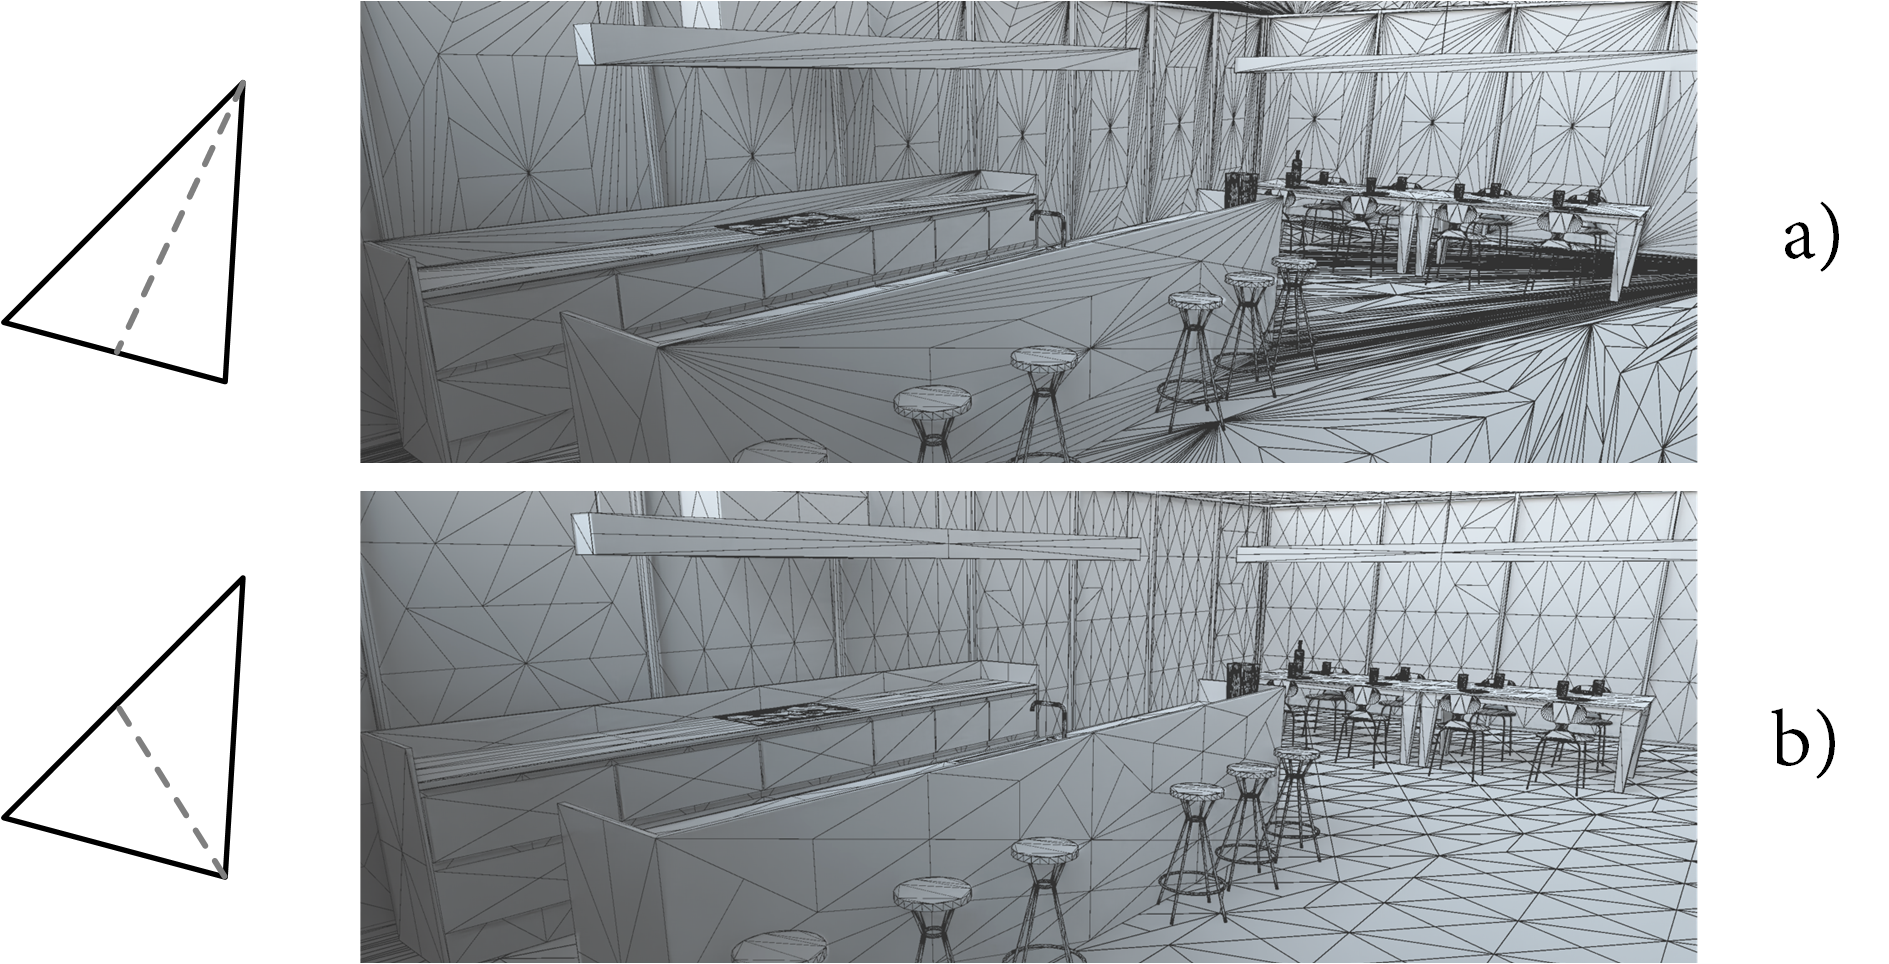
\includegraphics[width=\linewidth]{figs/lidar_optimization/triangle_subdivision.png}
	\caption{Two different triangle subdivisions over the same scene. a) Triangles subdivided by iterating through the edge to be split, and b) triangles subdivided with the proposed method.}
	\label{fig:triangle_subdivision}
\end{marginfigure}
Several approaches are effective to subdivide polygons, although some of them yield aesthetic results (see Figure \ref{fig:triangle_subdivision}). Whether the edge to be split is selected randomly, the triangle can be subdivided into large triangles that degenerate into segment-like polygons. This hardens the detection of collisions in the later ray-casting LiDAR, together with the loss of precision from using floating point data. Instead, the longest edge within each triangle can be split, thereby generating triangles with uniform edge lengths.

\section{Solution encoding}

\begin{marginfigure}[.2cm]
    \centering
    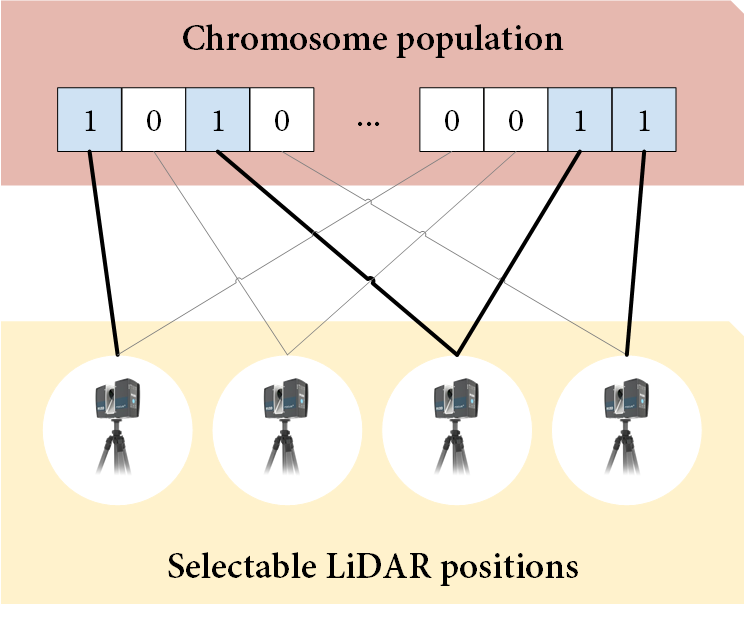
\includegraphics[width=\linewidth]{figs/lidar_optimization/solution_encoding.png}
	\caption{Binary encoding of active LiDAR solutions for a genetic algorithm.}
	\label{fig:solution_encoding}
\end{marginfigure}
Candidate solutions in GA are encoded as a buffer of binary values indicating which minimal set of LiDAR positions will be used for scanning. Each binary value is defined as an activation, whether this location will be a LiDAR position or not in the final setup. Firstly, positions are either uniformly or randomly sampled along the selected building level. Then, these are optimized with small changes whose effect will be measured with a metric. Finally, the GA is conducted to minimize the number of TLS scans while maximizing the coverage of a LiDAR point cloud.

With this sequence in mind, initial solutions are stored as $xyz$ coordinates, whereas the solutions of a GA are encoded as vectors of binary values $[b_0, b_1, b_2, ..., b_{k-1}]$, where $b_i \in \{0, 1\}$ and $k$ is the number of solutions generated on the previous spatial search. Although triggering $k$ solutions provide the most complete scan, the GA is intended to minimize the time required by human operators for scanning. Figure \ref{fig:solution_encoding} shows the proposed solution encoding for GAs. Binary values can be represented by Boolean data in the CPU; however, this data type is not uniformly represented in CPU and GPU hardware in terms of size, thus disallowing valid data transfers. Instead, Boolean values can be expressed using a minimal integer encoding in the GPU hardware with \verb|uint8_t| data type. In the GPU, it requires using the recent GLSL \verb|GL_NV_gpu_shader5| extension. Representations with a lower memory footprint are feasible with bit-level encoding, at expense of more intricate operations in accesses and modifications. Nevertheless, the algorithm configurations that are later presented allocate a few \verb|MBs| at most.

\section{Metrics}

Fitness functions are intended to evaluate the quality of candidate solutions to enable their optimization and determine which are the best for a specific setup. In this section, solutions are $n$ different positions located in the same building level, which are analysed from the perspective of four metrics. First, the number of scanned polygons provides a naïve measure regarding the coverage of the scenario ($F_1$: LOC). Also, polygons must be scanned with multiple points uniformly sparsed ($F_2$: LOD, LOA, LOC). Finally, TLS scans must meet a minimum overlapping factor that guarantees their fusion during post-processing ($F_3$: LOO). 

\subsection{Level of accuracy, coverage and resolution}

The LOC metric is trivially solved by counting the number of scanned polygons. However, measuring the uniformity of a point cloud is not as trivial. Instead of providing the desired resolution as a user-defined parameter, it can be computed during the pre-processing stage. Hence, a nearly optimal average is computed for each polygon by considering the average distance between uniformly sparsed points. These points can be retrieved from the parametric values of a triangle, $u$ and $v$, from a uniform distribution. Therefore, the polygons whose mean distance is higher than the reference mean are evaluated with a worse fitness value that contributes to the overall fitness. Regarding uniform distributions, QMC (Quasi-Monte Carlo) samplers approximate better what is expected from a randomized, yet uniform, scan. As a result, point clouds covering a polygon only with a few points are heavily penalized (Figure \ref{fig:f2_metric}). 

\begin{figure}
    \centering
    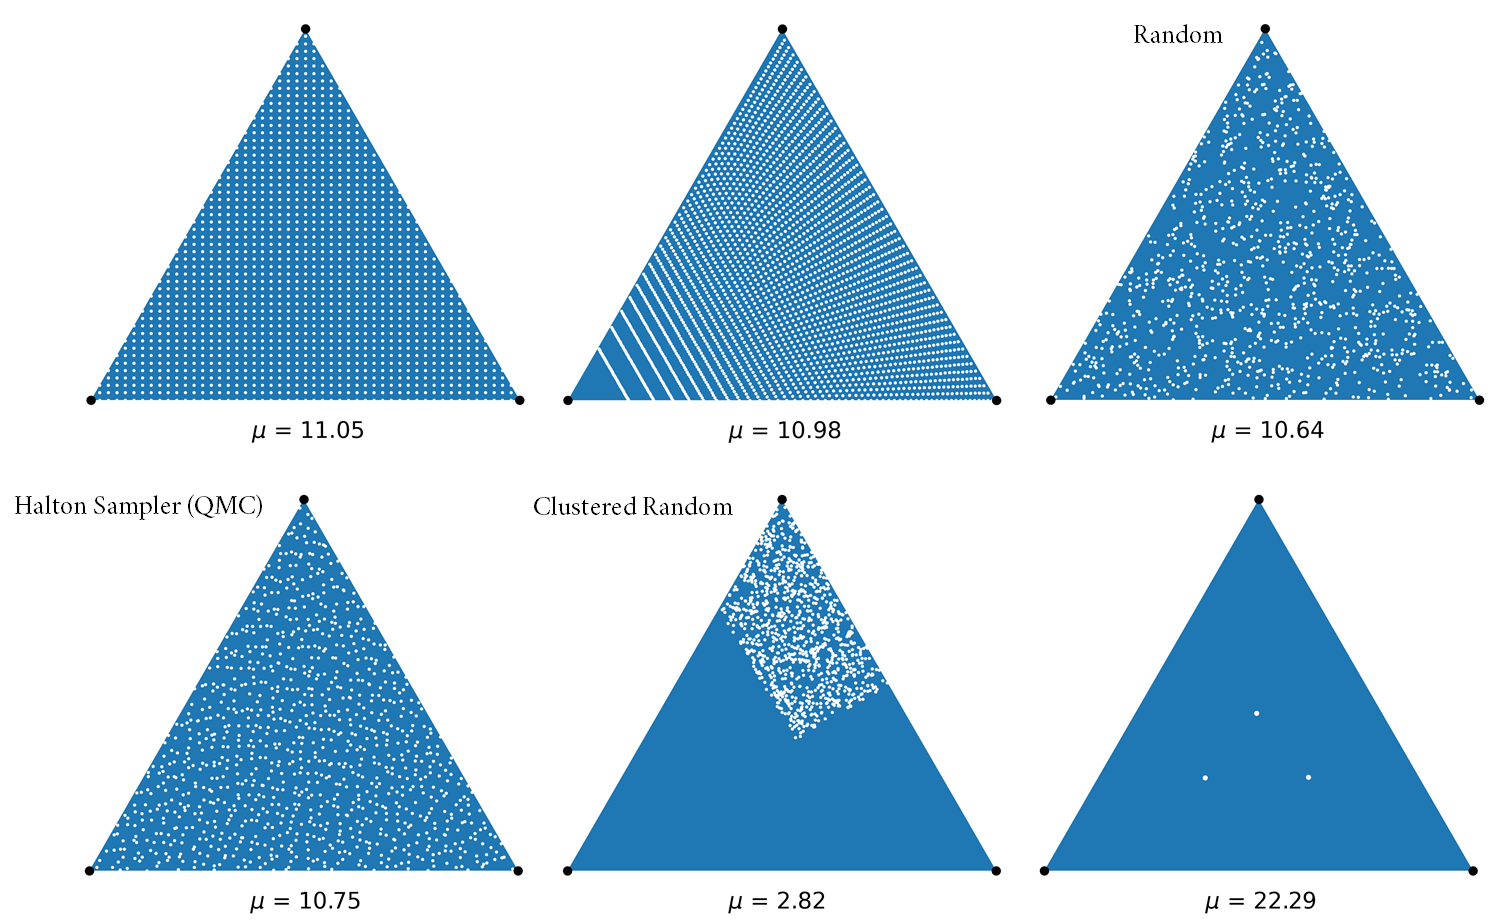
\includegraphics[width=\linewidth]{figs/lidar_optimization/distance_metric.png}
	\caption{Average distance ($\mu$) of every sampled point with the rest. From left to right, and from top to bottom: uniform grid distribution, uniform random sampling of $u$ and $v$, random distribution, QMC random distribution, random distribution only for a part of the triangle and three points uniformly scattered.}
	\label{fig:f2_metric}
\end{figure}

Both $F_1$ and $F_2$ metrics allow enhancing starting positions by translating them towards better locations, and they can be applied to one or multiple scans. In terms of preferences, point cloud uniformity and accuracy are typically preferred over coverage for a single scan. However, the latter metric can be trivially approached by selecting the subset of points that guarantee appropriate coverage. Despite this, $F_1$ and $F_2$ are considered during optimization, with $F_1$ working as a secondary metric that enables untying solutions of equal fitness. These are defined as shown in Equations \ref{eq:metric_count} and \ref{eq:uniformity_error} for evaluating a set of solutions, $K$. Individual solutions present a buffer of collided triangles, $T$, with each one being collided by a set of points, $P$. The set of collided triangle indices is here denoted by $L$, with each index appearing only once, whereas every possible triangle is noted as $S$.

\begin{align*}
    \textit{F}_{1} &= \sum_{s=1}^{\abs{S}} 1[t_s \in \{L_1, L_2, ..., L_k\}]
    \numberthis \label{eq:metric_count}\\
    \textit{F}_{2} &= \sum_{k=1}^{\abs{K}} \left(\sum_{s=1}^{\abs{S}} d_{\textit{optimal}_{s}} - \sum_{l=1}^{\abs{L_k}} d_{\textit{optimal}_{l}}  +\right.\\ & 
    \left. + \sum_{t=1}^{\abs{T_k}} \left(\frac{\sum_{i=1}^{\abs{P_t}} \frac{\sum_{j=1}^{\abs{P_t}} d^{2}(p_i, p_j)}{\max\left(\abs{P_t} - 1, 1\right)} \cdot (2 - \abs{\widehat{n}_{t_{k}} \cdot \widehat{\left(r_{o} - p_{i}\right)}})}{\max\left(\abs{P_t}, 1\right)} - d_{\textit{optimal}_{t}}\right)\right)
    \numberthis \label{eq:uniformity_error}
\end{align*}
where $F_1$ represents the number of different intersected polygons and $F_2$ estimates the accuracy by measuring the distance from the optimal uniformity to the computed one. $d$ represents a distance function, e.g., the Euclidean, $t_s$ is a triangle index in $S$, $\hat{n}$ is the normal vector of a triangle, and $r_o$ is the sensor eye. Instead of solely accounting for the distance from intersected primitives, $F_2$ also sums the distance from non-collided polygons. However, the distance from intersected polygons must be subtracted to avoid penalizing solutions with a higher number of collisions (Figure \ref{fig:f2_sampling}). Remark that $F_2$ intends to minimize the measured distance. Therefore, the number of reached polygons, $F_1$, is somehow considered in this formula by penalizing scans that only reach a small number of polygons.

Also, note the sensor's range is frequently integrated into the LOA metric by discarding returns whose distance is above the maximum allowed distance. However, these criteria can be integrated during the LiDAR simulation, rather than worsening the efficiency of $F_2$ estimations. Following this approach, the range of the LiDAR can be severely reduced to consider only close returns, thus accounting for its accuracy, despite real simulations providing denser scans. 

\begin{figure}
    \centering
    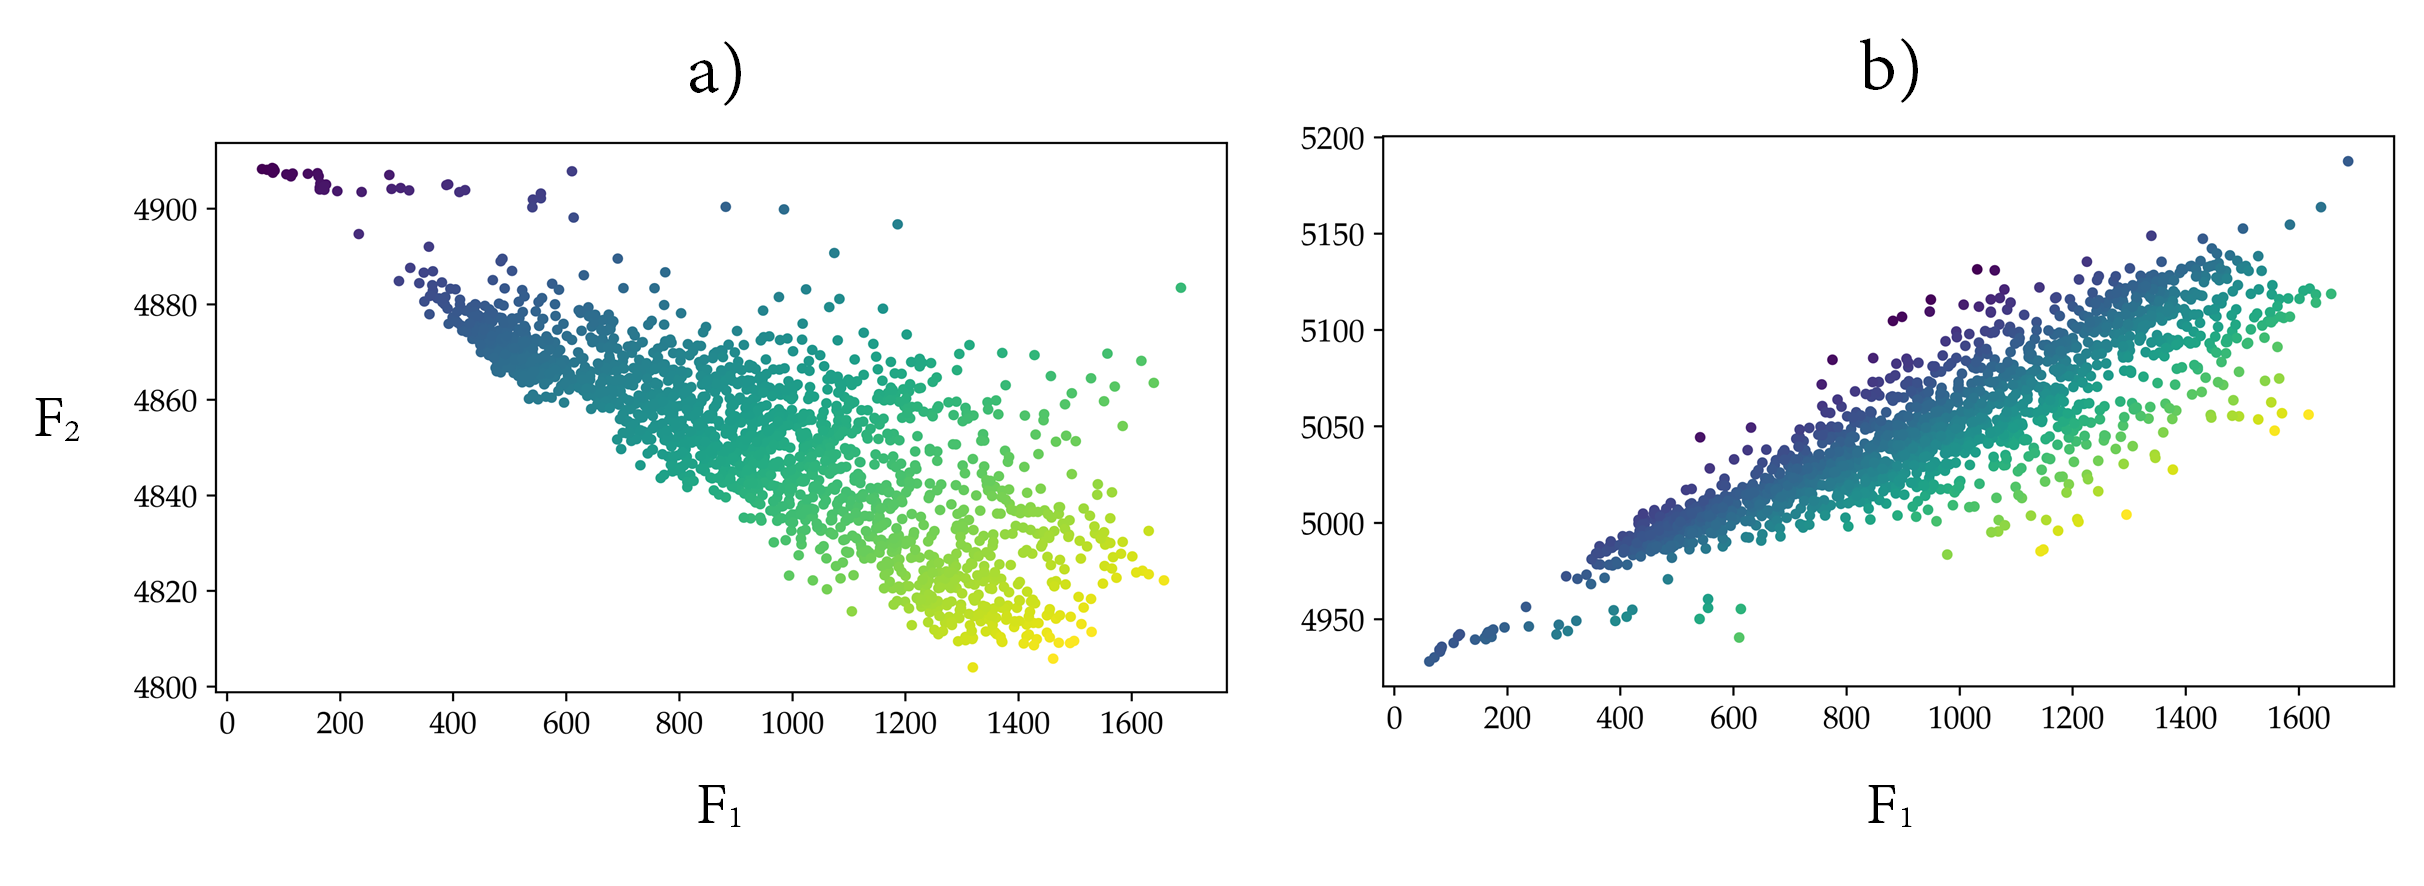
\includegraphics[width=\linewidth]{figs/lidar_optimization/f2_sampling.png}
	\caption{$F_1$ and $F_2$ obtained by uniformly sampling a 3D environment. The first image depicts the results of $F_2$ as proposed (minimization of $F_2$ and maximization of $F_1$). The second plot is obtained by not removing the default distance of collided polygons.}
	\label{fig:f2_sampling}
\end{figure}

\subsection{Level of overlap}

The $F_2$ metric is better suited for achieving local improvements, whereas $F_1$ fits better on the selection of the minimum number of locations providing better scene coverage. However, none of these metrics considers the overlapping of individual scans, despite it being required to guarantee their alignment in post-processing. To this end, features which are visible in a scan must appear in others. With this objective, the $F_3$ metric defined in Equation \ref{eq:overlap_metric} measures the overlapping area between two LiDAR scans, indexed as $i$ and $j$, and depicted as circumferences with a fixed radius, $r$.  

\begin{align*}
    A_{i, j} =& \left(r_{i}^{2} \cos^{-1}(\frac{d_i}{r_{i}}) - d_i \sqrt{r_{i}^2 - d_{i}^{2}} +\right. \\
    &\left.+ r_{j}^{2} \cos^{-1}(\frac{d_j}{r_{j}}) - d_j \sqrt{r_{j}^2 - d_{j}^{2}}\right)\\  
    A_{i, j, r_i = r_j} =& 2\left(r^{2} \cos^{-1}(\frac{d}{2r}) - \frac{d}{2} \sqrt{r^2 - \left(\frac{d}{2}\right)^{2}}\right)\\
    \textit{F}_{3_{i, j}^\theta} =& \frac{A_{i, j}}{\pi r_{i}^2} \hspace{1mm} | \hspace{2mm} i, j = 1, 2, ..., \abs{P_c}
    \numberthis \label{eq:overlap_metric}
\end{align*}
where $d = d_i + d_j$, $d$ is the distance from two locations and $r$ is the LiDAR maximum range, which was previously clamped to account for the accuracy loss from distance. $r$ is the same for every scan, thus leading to $d_i = d_j$.

\begin{marginfigure}
    \centering
    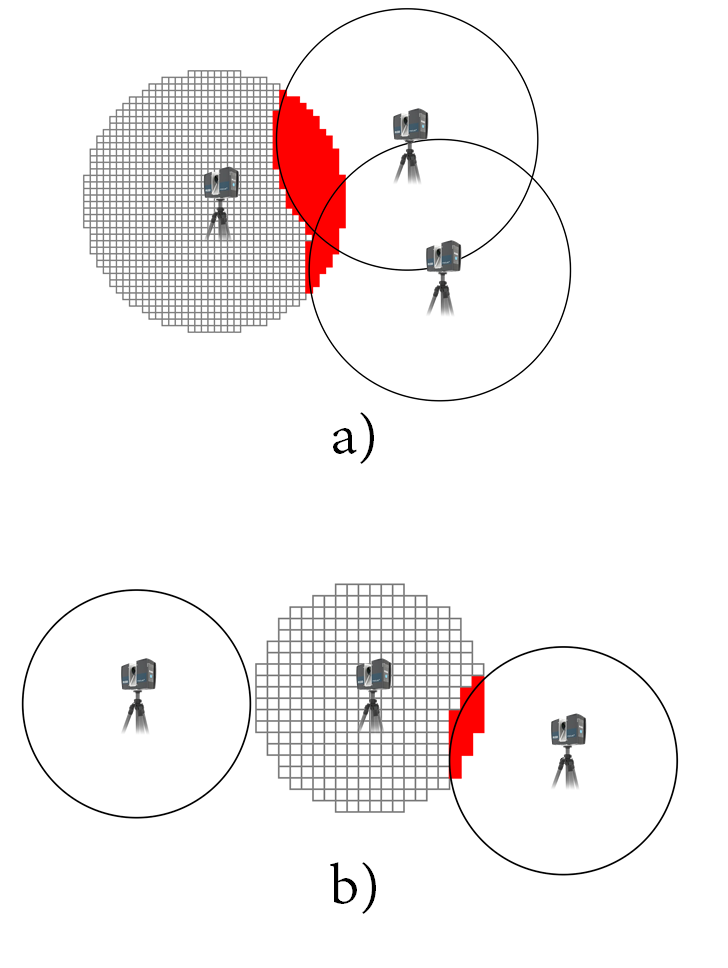
\includegraphics[width=.8\linewidth]{figs/lidar_optimization/loo.png}
	\caption{Grid occupancy in two different configurations. a) Grid with higher resolution and three overlapping circumferences, and b) sparser grid with only two overlapping circumferences.}
	\label{fig:loo_example}
\end{marginfigure}
The main drawback of Equation \ref{eq:overlap_metric} is that it does not account for the overlapping of previously added locations. To handle this, the occupancy of each LiDAR scan is represented using a 2D grid that is filled with points sampled from other scans. Hence, the estimated overlap is given by the number of voxels occupied with respect to the total number. If $d \geq d_1 + d_2$, then sampling can be omitted since both locations do not overlap. Yet, Equation \ref{eq:overlap_metric} helps to establish a ranking of candidate solutions, thus measuring how helpful are these to achieve the required overlapping. However, ranking locations by their overlapping leads to selecting those with the highest overlap instead of the required one. Accordingly, Equation \ref{eq:loo} ranks locations by their distance to the required overlap. However, solutions that offer a higher overlap than the required one are preferred over those below. To guarantee this, the most significant bit of preferred locations is set to one. Due to the sampling strategy, the accuracy of the overlapping estimations depends on the grid subdivision as well as on the number of sampled points belonging to another TLS scan, as depicted in Figure \ref{fig:loo_example}.
\begin{align*}
    \textit{F}_{3_{i, j}} &= r - \abs{\psi - \textit{F}_{3_{i, j}}}\\
    \textit{F}_{3_{i, j}} &= \textit{F}_{3_{i, j}} \BitOr{1 \ShiftLeft 32} \hspace{3mm} \textit{if} \hspace{1mm}  \textit{F}_{3_{i, j}} \geq \psi
    \numberthis \label{eq:loo}
\end{align*}
with $\psi$ being the required overlapping percentage.

Following this approach, the required overlapping is guaranteed for every solution. Still, another shortcoming is the appearance of disjoint sets as a result of selecting the best $n$ solutions with greedy algorithms. Analogously, this drawback can be identified using a data structure called a disjoint set. New solutions are attached to this structure until there is a single disjoint set. These are added according to their distance to another disjoint set and the value of $F_3$, as proposed in Equation \ref{eq:disjoint_set_metric}. The procedure to join disjoint sets is the following:
\begin{itemize}
    \item First, the closest disjoint sets are selected, as well as the two closest solutions within both of them.
    \item Then, solutions overlapped with the first location are sorted according to the maximization problem evaluated by Equation \ref{eq:disjoint_set_metric}. 
    \item The new LiDAR location is linked to the first solution, which is known to be overlapped, whereas the second solution is only liked whether the overlapping is higher than zero. 
    \item New solutions are also checked to guarantee the required overlapping.
\end{itemize}
\begin{align*}
    g(p_o, p_d, p_i) = \left(\frac{d(p_o, p_d) - d(p_i, p_d)}{d(p_o, p_d)} \textit{F}_{3_{o, i}}\right)
    \numberthis \label{eq:disjoint_set_metric}
\end{align*}

\subsection{Point sampling}

During this preprocessing stage, polygons are iteratively sampled to generate uniformly distributed point clouds. Then, the mean distance within a single triangle is computed as shown in Equation \ref{eq:mean_distance}. The Euclidean distance, although it could be exchanged with any other distance-based function. Note that $\abs{P}-1$ is used instead of $\abs{P}$ to not take into account the distance of points with themselves in an efficient way. 
\begin{align*}
    d_{\mu} = \frac{\sum_{i=1}^{\abs{P_t}} \frac{\sum_{j=1}^{\abs{P_t}} d^{2}(p_{i} - p_{j})}{\max\left(\abs{P} - 1, 1\right)}}{\max\left(\abs{P}, 1\right)}
    \numberthis \label{eq:mean_distance}
\end{align*}
where $P_t$ represents a set of points within a triangle $t$, whereas the inner summation computes the Euclidean distance for 3D points.

\begin{marginfigure}[-5cm]
    \centering
    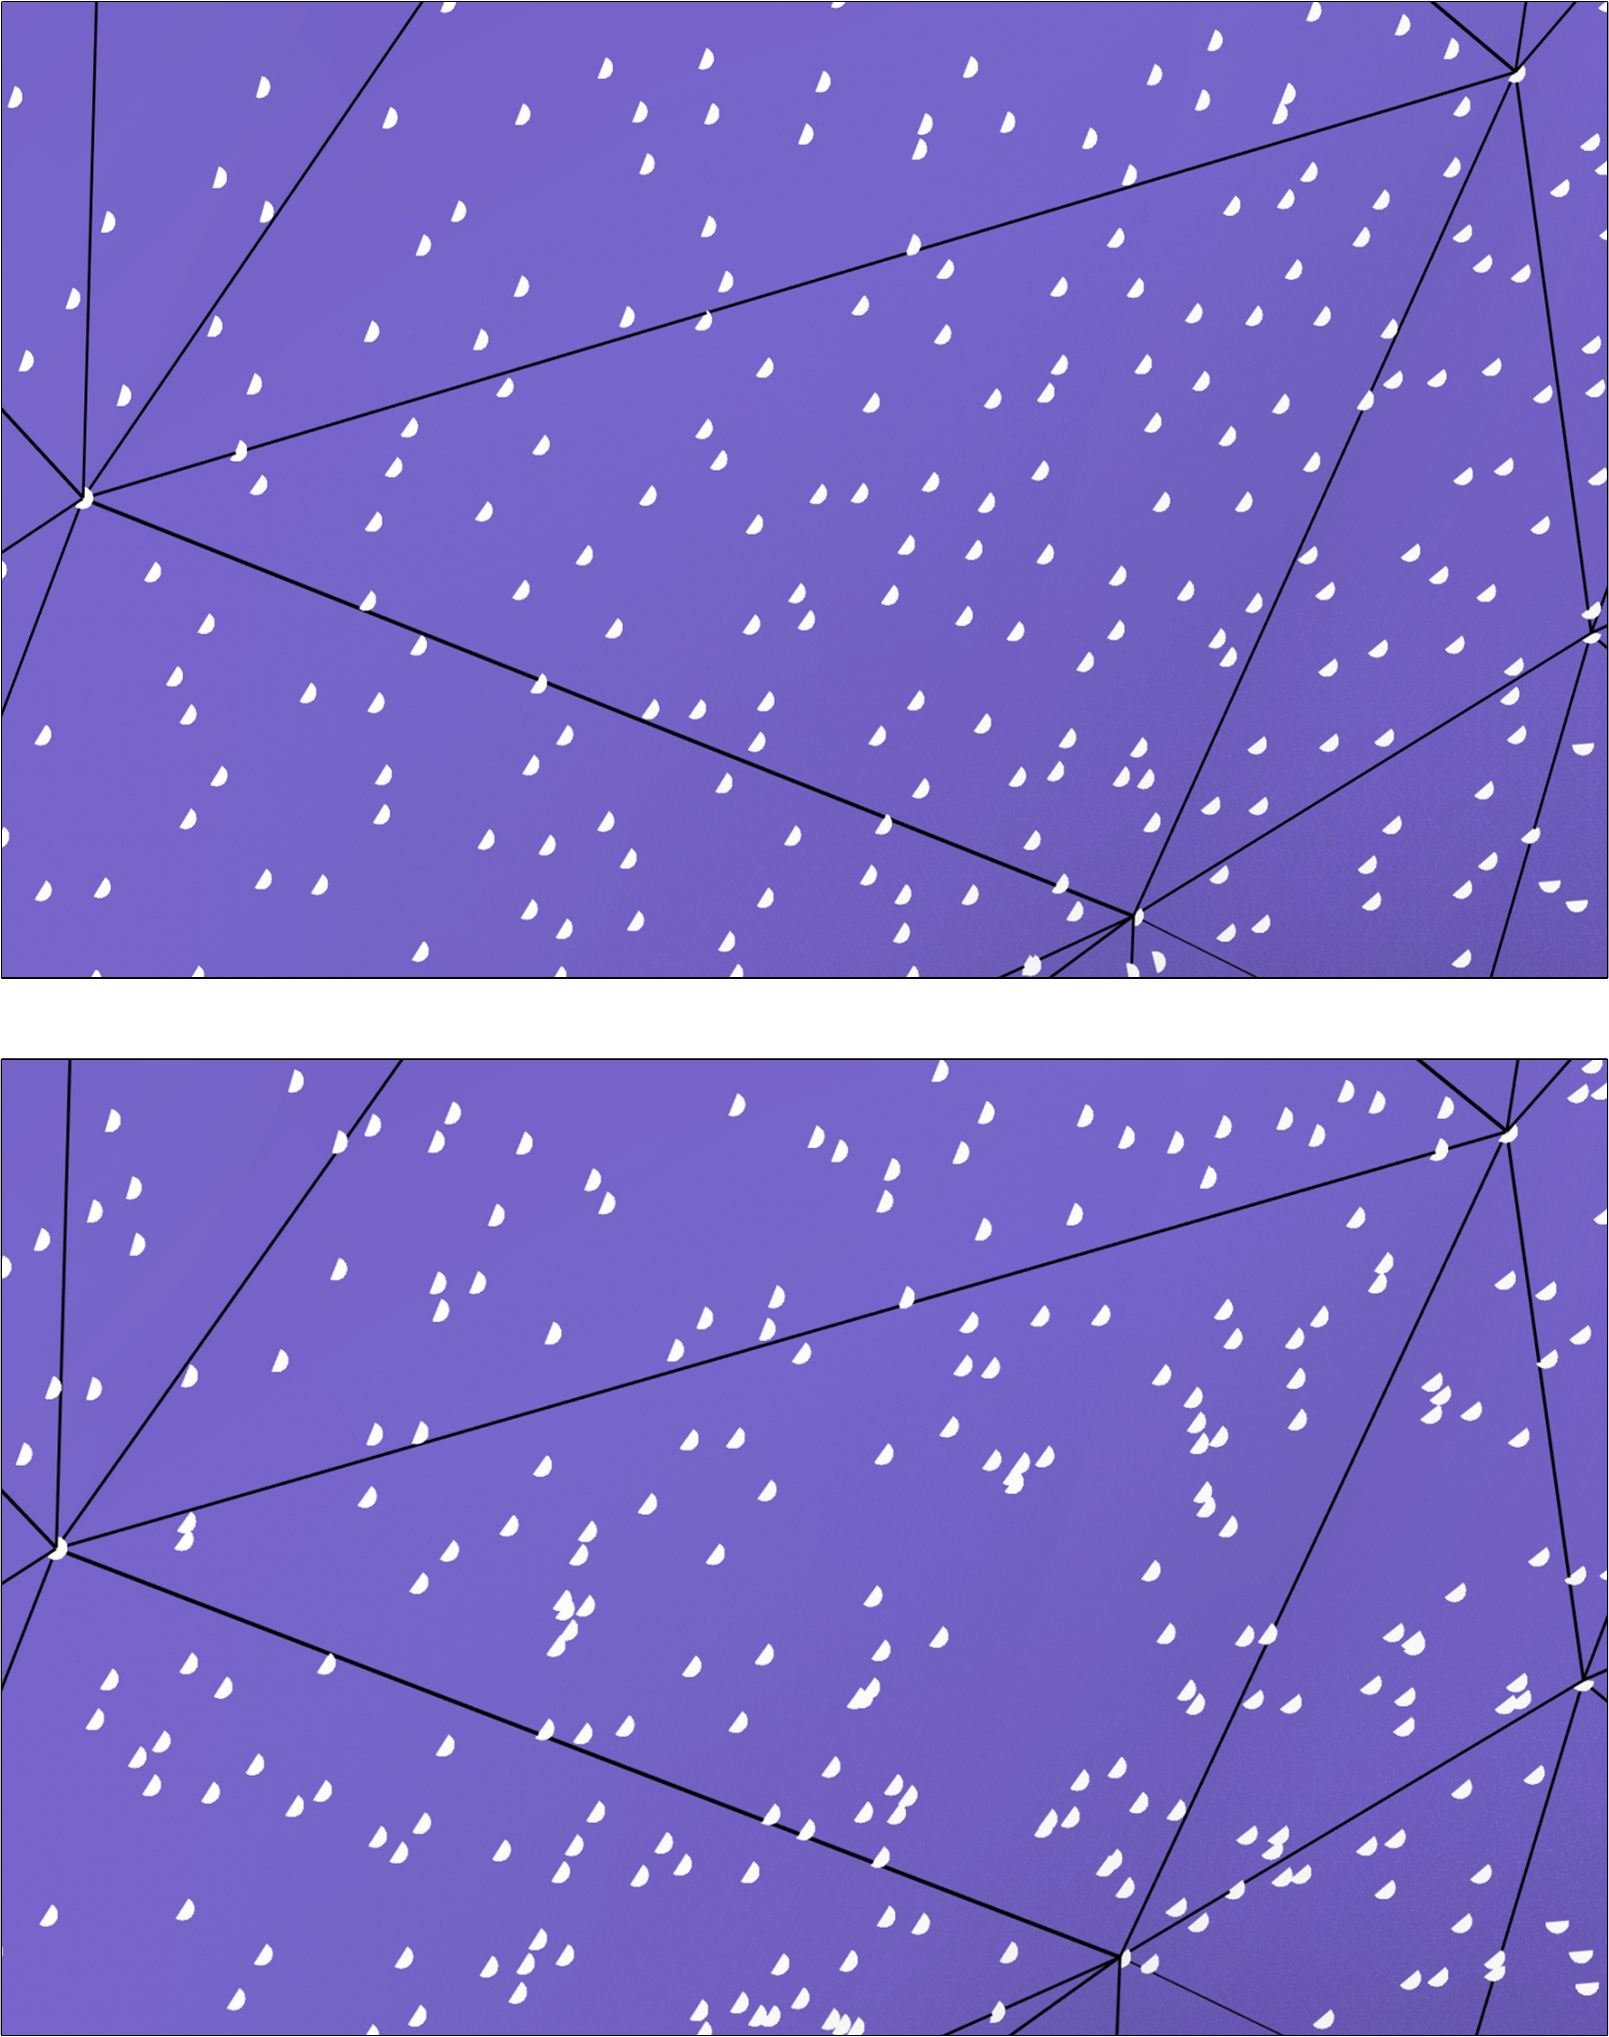
\includegraphics[width=\linewidth]{figs/lidar_optimization/point_sampling.png}
	\caption{Comparison of polygons sampled using the Halton sequence (more uniformity) and the C++ built-in random uniform distribution.}
	\label{fig:point_sampling}
\end{marginfigure}
Despite there exist built-in random uniform distributions in most language libraries, these are mainly based on pseudo-random sequences, such as those used for Classic Monte Carlo integration (CMC). They provide good quality estimations, but they require a large number of samples and have a higher response time \cite{marques_optimal_2019}. The response time is irrelevant in this case study since we solely sample a few points from each triangle, where the number depends on the polygon area. However, these distributions generate point clouds far from the expected uniformity. Instead, the QMC method is based on well-distributed deterministic sampling patterns that provide better results for our objective. More specifically, the Halton sequence was used to calculate the quasi-optimal mean distance within polygons \cite{burkardt_halton_2010}. Figure \ref{fig:point_sampling} shows the results of sampling with both the C++ built-in random uniform distribution and the proposed QMC sequence.

Either from pseudo-random or QMC sequences, two parametric values ($u$, $v$) are generated to sample a triangle surface. Equation \ref{eq:triangle_parametric} shows the formula for generating a point within a triangle defined through its three vertices ($p_1$, $p_2$, $p_3$) with $u, v \in [0, 1]$. 
\begin{align*}
    p_{s} = (1 - \sqrt{u}) p_1 + (\sqrt{u} (1 - v)) p_2 + (v \sqrt{u}) p_3
    \numberthis \label{eq:triangle_parametric}
\end{align*}

Note that a significant drawback of this approach is that sparse scans with all their points gathered in a small area are also evaluated as appropriately uniform. To solve this, the triangle vertices were included as part of the point set, $\abs{P}$, thus penalizing scans biased towards certain parts of polygons.

\subsection{Solution initialization}

A continuous 3D space must be discretized to obtain the initial solutions, $N$, over polygons that are interactively marked as ground. From the collected ground planes, the 2D axis-aligned bounding box (AABB) is computed to restrict the instancing area. Still, this approach may lead to generating points that fall out of ground-labelled polygons for non-rectangular ground surfaces. Therefore, candidate locations are evaluated in the GPU to verify that:
\begin{itemize}
  \item \textbf{The location is over a ground polygon}. To verify this, a ray is cast towards -\textit{Y} in the BVH. Ground polygons are transferred to the GPU and their ID is compared against the nearest collision.
  \item \textbf{The sensor is not located over non-ground planes}, e.g., furniture placed between the floor and the LiDAR sensor. \textit{m} points are sampled around the candidate location, using a radius $r$ and casting $m$ rays with $-\vec{Y}$ direction. The location is discarded whether any of the $m$ rays have their nearest collision in non-ground-labelled items. Both $r$ and $m$ can be configured.
  \item \textbf{The sensor is not located close to building walls and furniture}. It cannot be placed over items, nor next to them, thus guaranteeing a safety distance ($d$). Hence, four additional rays are cast using \{\textit{X, -X, Z, -Z}\} vectors.
\end{itemize}

Candidate solutions can be generated with random or uniform sampling. Uniform sampling is supported by a 3D matrix bounded by the ground 2D AABB, whereas the height is limited by the LiDAR's maximum and minimum height. The level of subdivision is parameterized with the voxel size, with lower sizes providing a better LOD and a larger dimensionality of $N$. Otherwise, solutions can be randomly distributed to provide a less exhaustive initialization. It explores fewer solutions, scattered throughout the scene by a random uniform distribution. Note that uniformity is not as helpful as before, and therefore it is avoided. Then, $N$ is either enhanced (spatial searches), subsampled (greedy algorithm) or narrowed with bit sets (GA). 

\section{Spatial search}

This section explains how are the initial solutions, $N$, improved, to provide a wider space exploration instead of simply relying on the starting locations. However, metrics aimed at improving scans do not have any knowledge concerning overlapping. The following searches work according to the $F_2$ metric from Equation \ref{eq:uniformity_error}.

\subsection{Solution neighbourhood}

\begin{marginfigure}[.cm]
    \centering
    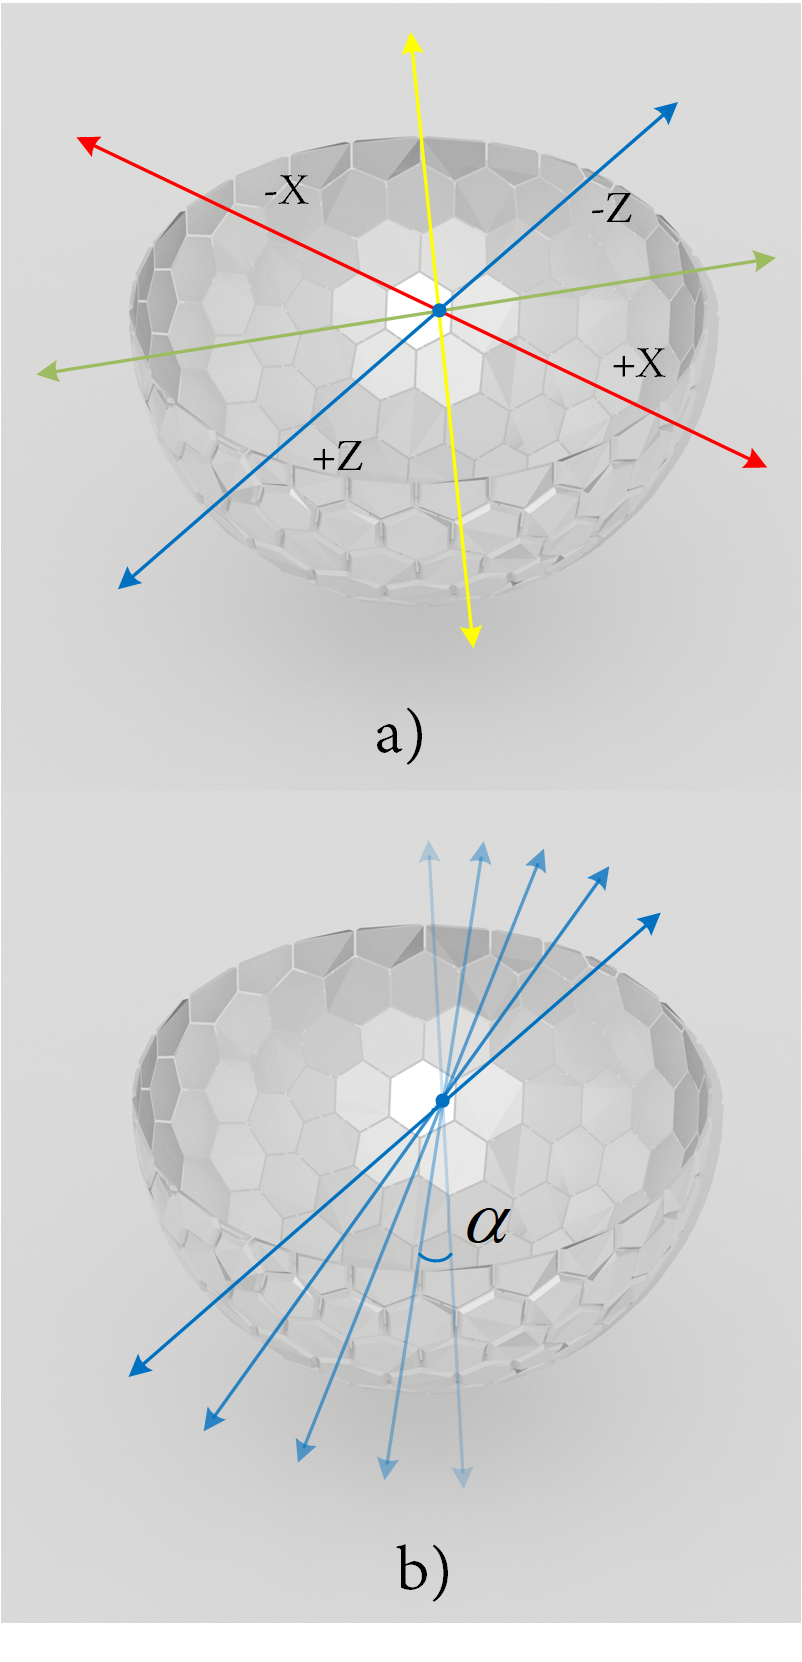
\includegraphics[width=\linewidth]{figs/lidar_optimization/neighbour_search.png}
	\caption{Overview of gradients for a 2D neighbour search. a) Constant approach that generates 8 vectors, whereas b) sub-samples the circumference according to a resolution parameter.}
	\label{fig:neighbour_search}
\end{marginfigure}
Neighbourhood exploration is introduced to locally enhance candidate locations. The neighbourhood is composed of 3D points near a sensor location. Its discretization poses several challenges since it there exists an infinite number of translation, despite being unitary. It can be discretized by downscaling the neighbours to 14 unitary vectors, given by the six faces and eight corners of a cube. Otherwise, it can be discretized by uniformly subsampling a unit sphere, thus obtaining a buffer of gradients whose length depends on the user-defined sampling resolution. Furthermore, unit vectors can be scaled by defining the step length; larger steps leads to omitting good candidates, whereas an extremely small length may be too exhaustive and not reach any improvement. Figure \ref{fig:neighbour_search} illustrates the gradient vectors that help to explore the contigous space in 2D: the first scenario have some fixed subdivisions, whereas the second depends on the given resolution.

%\begin{figure}
%    \centering
%    \includegraphics[width=\linewidth]{figs/png/GreedyTeaser.png}
%	\caption{Output of a greedy algorithm, selecting 20 locations out of uniformly distributed 30 points.}
%	\label{FIG:GreedyTeaser}
%\end{figure}

\subsection{Greedy algorithm}

The traditional local search is here referred as a Greedy algorithm that helps to rapidly survey the neighbourhood. These surrounding points are evaluated and sorted according to its fitness. Solutions are iteratively improved by moving to the best found solution, if any improves the current fitness. Otherwise, this approach gets stuck on a local minima and terminates. The termination criteria also contemplates reaching a maximum number of iterations. Re-visiting previous explored locations is avoided with an efficient $\textit{dot}$ product of the gradient being evaluated and the previous one ($f(\hat{g}_1, \hat{g}_2) = \hat{g}_1 \cdot \hat{g}_2$). A gradient is considered to be already explored whether $f(\hat{g}_1, \hat{g}_2) < \epsilon - 1$, with $\epsilon$ being a small value such as $2^{16}$ that avoids errors in comparisons with floating-point data. Remark that this efficient check tackles inmediately revisiting previous neighbours, though it could enter in a more intrincate cycle loop.

\subsection{Simulated Annealing}

Simulated snnealing, in contrast to the greedy approach, implements some mechanism to avoid getting stuck in local optima. To this end, neighbours with worse fitness than the current solution are accepted under probabilistic criteria. A temperature value ($T$) is first initialized and reduced iteratively, with the acceptance rate of worse solutions being lower as $T$ decreases (cooling) \cite{wieckowski_finding_2020}. In this work, it is configured using the traditional exponential formula defined in Equation \ref{eq:simulated_annealing_exp}: 
\begin{gather}
    \label{eq:simulated_annealing_exp}
    \begin{aligned}
        p(f') =
        \begin{cases}
            \exp(\frac{f'-f}{T}) &f'-f \geq 0\\
            1 &f'-f < 0
        \end{cases}
    \end{aligned}
\end{gather}
given that $f'$ and $f$ are two fitness values from a new solution and the current one, respectively, in a minimization problem. Consequently, a random uniform distribution is also applied to determine whether a worse solution is accepted. The stop criterion depends on a threshold temperature and a maximum number of iterations.

\subsection{Tabu search}

A trivial improvement of local search is the tabu search, where the already processed locations are stored as the so-called tabu moves. These cannot be explored again, which may lead to all the neighbours being tabu. In this case, the solution space is re-initialized. This scenario is also achieved when every neighbour worsen the fitness value obtained from the current location and the best one, or a maximum number of iterations is reached without any improvement. The main challenge in 3D is how to handle these tabu moves, which were here approached using a 3D regular grid of variable resolution. Then, a neighbour is considered tabu when the target point falls in a tabu voxel. Given the step size of neighbour explorations, $n_l$, an appropriate voxel size is given by $f \cdot n_l$, with $1 < f < 2$.

\section{Genetic algorithm}

\begin{marginfigure}[-6.0cm]
    \centering
    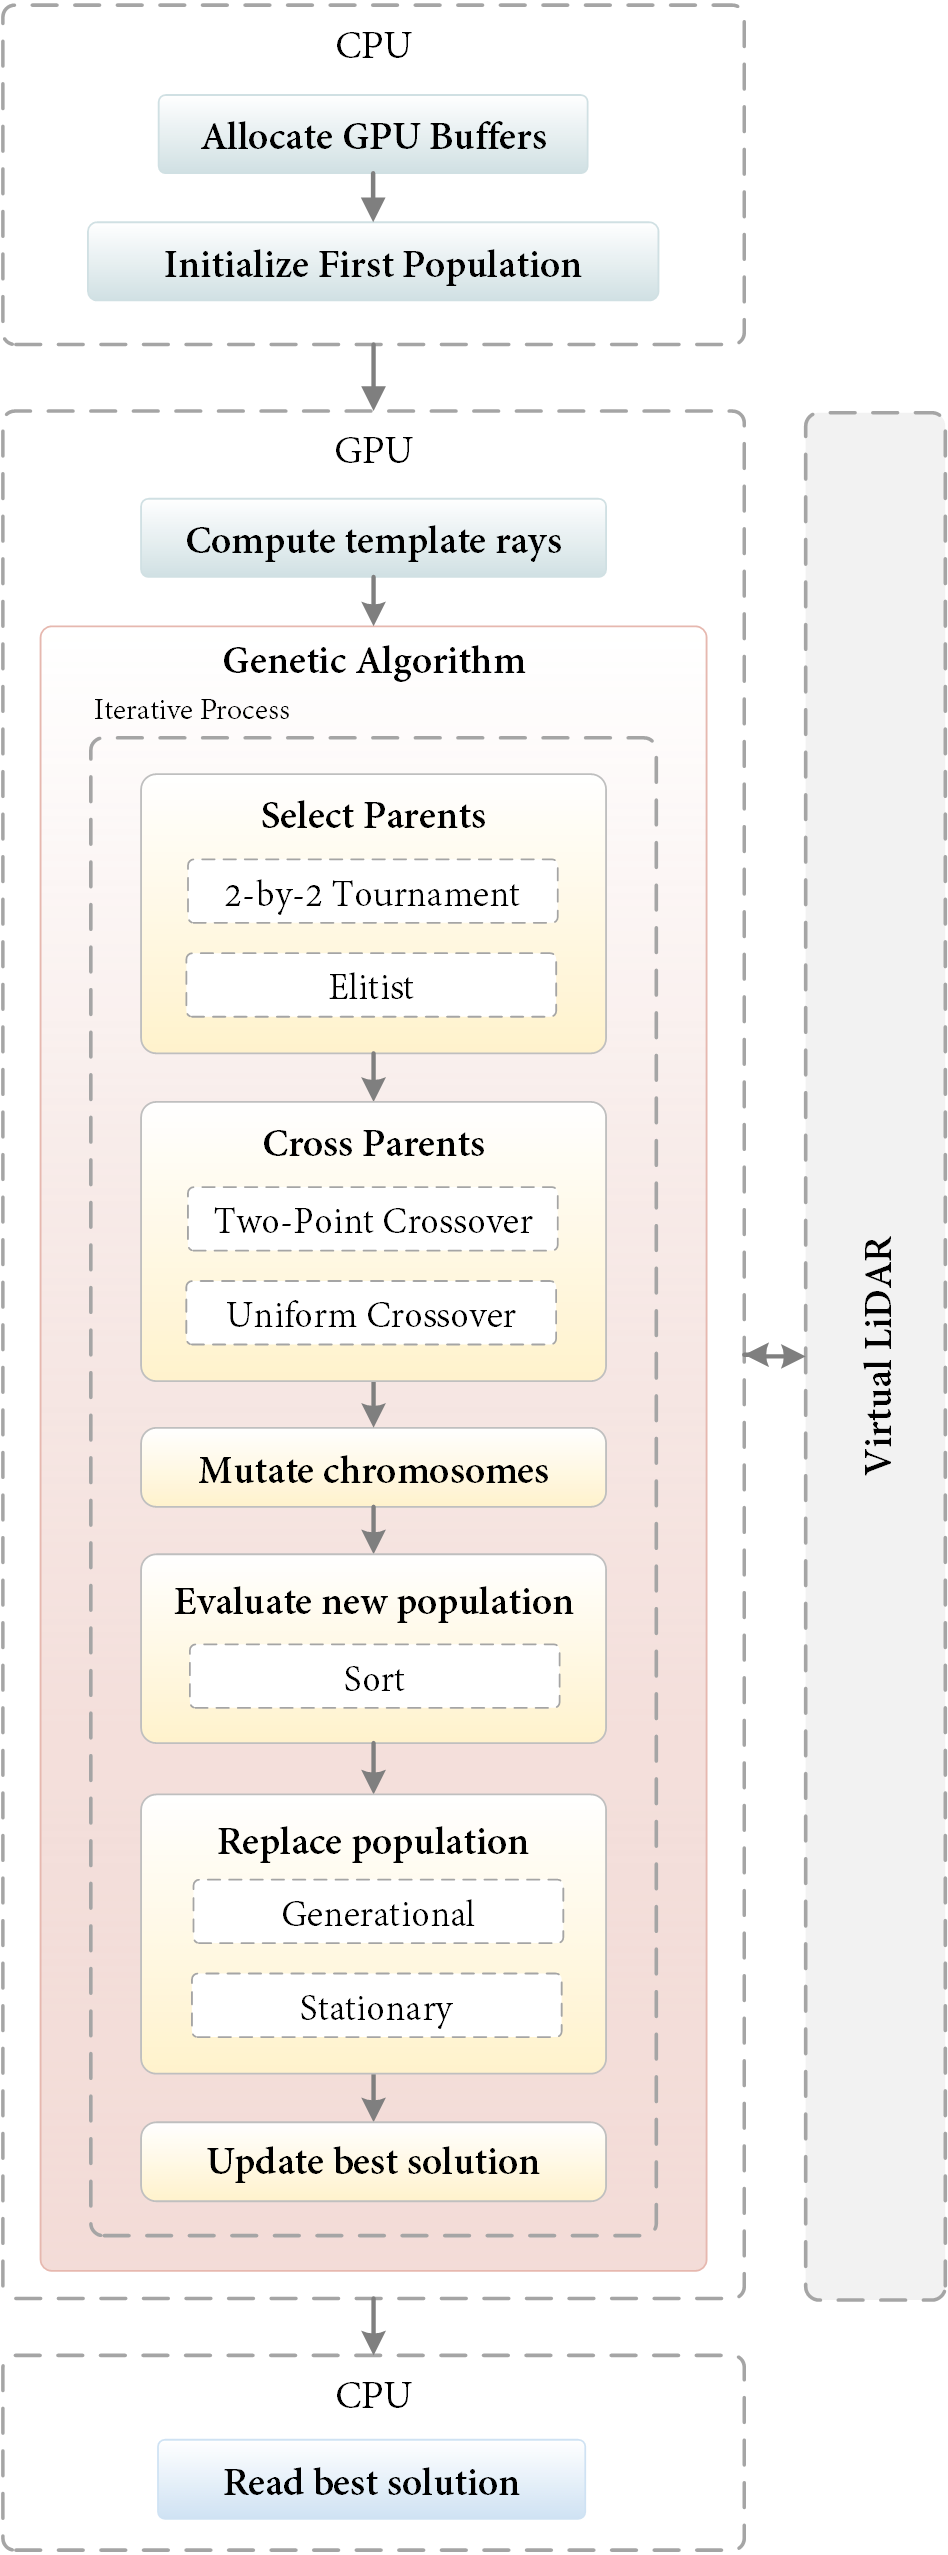
\includegraphics[width=\linewidth]{figs/lidar_optimization/genetic_overview.png}
	\caption{Overview of GAs in the evaluation of the best combination of spatial LiDAR setups.}
	\label{fig:genetic_overview}
\end{marginfigure}
Genetic algorithms operate over the previously enhanced solution to find an optimal subset. This sort of algorithm is inspired by nature on how to handle populations that evolve and improve over time. Accordingly, it combines exploration and exploitation phases \cite{vannucci_genetic_2020}. Regarding our case study, this metaheuristic helps to reduce the setup complexity while still providing a dense coverage. In comparison with memetic algorithms, the first stage aims to improve individual locations guided by an exploration of surrounding areas, without evaluating the scene coverage. Still, the proposed $F_2$ metric weights non-scanned polygons. After this, a GA finds the optimal solution regarding the scene coverage. 
To this end, a slight variation of the previously proposed $F_1$ metric is here proposed. 
The complete procedure is depicted in Figure \ref{fig:genetic_overview}, whose stages are following detailed:

\textbf{Initialization of population}. The population is first generated with $p$ chromosomes of size $n$, each one with a random number of activations (LiDAR locations). Hence, variety is ensured by avoiding populations with a fixed number of activated bits.

\textbf{Compute template rays}. Template rays are first built to describe how rays traverse the space from a default LiDAR location, which is known to be at $0^3$. These rays are generated according to the specifications of a commercial LiDAR sensor. Then, the LiDAR point clouds are simulated from this set of rays. Template rays are only transferred once to the GPU, rather than calculating and transferring them for every location to be checked. The GPU-based LiDAR simulation proposed in previous chapters was simplified to provide only the first collision to favour both replicability and performance. 

\textbf{Parent selection}. The aim of this stage is to select the $s$ most promising individuals for the subsequent crossover. Two different selections are here proposed. First, the 2-by-2 tournament allows selecting good solutions, though they may not be within the top-most $s$. Therefore, this leads to introducing some minor variety into later populations. Otherwise, the elitist approach selects the best individuals from the current population.

\textbf{Crossover}. Previously selected parents are combined to generate the next population. Parents can be mixed by selecting a crossing point, thus generating two gen chunks for each parent, which are combined to build offspring. Another approach is to process gens individually by retrieving uniformly distributed random values which determine the parent ($p_{1_{i}}$ if $r_i \leq 0.5$, $p_{2_{i}}$ otherwise). There is only a non-valid solution, the zero chromosome ($0^n$), which is easily tackled by randomly altering a single bit.

\textbf{Mutation}. Mutation enables including minor variations are introduced in the new generation. This process is parameterized by the number of mutable individuals and genes within each one. There is not any restriction concerning the number of activations, and therefore, mutations can be performed by randomly activating or deactivating some bits.

\marginnote[.5cm]{
	\begin{equation}
    \textit{F}_{1} = \frac{\sum_{s=1}^{\abs{S}} 1[t_s \in \{L_1, ..., L_k\}]}{\sum_{g=1}^{n} c_g}
    \label{eq:metric_count_alt}
	\end{equation}
}
\textbf{Evaluation of new population}. The fitness of every new solution is estimated based on the computed returns. Accordingly, solutions covering more polygons are more likely to be selected as parents in the following iterations. However, this approach leads the population to activate every bit. For this reason, the previously proposed $F_1$ metric is modified according to Equation \ref{eq:metric_count_alt} by also accounting for the number of activated bits within a chromosome ($c_g$). With this new metric, the genetic algorithm is intended to reach the maximum number of polygons with the minimum number of scans.

\textbf{Replace population}. New and previous populations are here mixed following a generational or stationary method. The generational approach replaces parents with their offspring, whereas the stationary algorithm replaces the worst individuals with the new population whether they improve current solutions.

\textbf{Update best solution}. It is noteworthy that even this minor operation must be performed in the GPU, as the reading transfer would lead to a huge delay in the GA response time.

\section{Interactive tools}

This section presents some tools intended to facilitate the configuration of the scenario and the algorithm.

\subsection{Level selection}

The described P4S method is not restricted to buildings with a single level. Indeed, it has been evaluated in realistic buildings with several of them, and yet, the planning must be performed individually. The selection of floor-labelled polygons is interactively performed through ray-casting, thus solving in real-time which one was picked. The result is computed by casting a ray whose direction is given by the user's viewpoint and a 3D position. This position is computed by unprojecting the camera matrix to a 2D point within the application canvas. The first collided model is obtained traversing the BVH, and pushed into the ground list. With this regard, Equations \ref{eq:unprojection1} and \ref{eq:unprojection2} show how to unproject a 2D canvas point to 3D.
\begin{align*}
    p_{\textit{3D}} &= \hspace{.5mm} \inv{\left(P \cdot V \cdot M\right)} \cdot \hspace{1mm} \left[\frac{p_{\mathit{2D}_x}}{c_x}2 - 1,  \frac{p_{\mathit{2D}_y}}{c_y}2 - 1, 0, 1\right]^T
    \numberthis \label{eq:unprojection1}\\
    p_{\textit{3D}} &= \frac{p_{\textit{3D}}}{p_{\textit{3D}_w}}
    \numberthis \label{eq:unprojection2}
\end{align*}
where $(p_{\textit{2D}_x}, p_{\textit{2D}_y)}$ is the canvas point, $P$, $V$ are the camera projection and view matrices, respectively, $(c_x, c_y)$ is the canvas size, and $p_{\textit{3D}}$ is a 4-tuple describing the projection coordinates.

\subsection{Pipeline design}

Spatial searches and GAs could be concatenated to iteratively improve the starting solutions. Hence, the explained pipeline is not limited to applying first a local search that is later narrowed with GAs. Instead, local searches could be omitted, several of them could be chained, or even the final reduction may be unnecessary whether scanning from a larger number of locations is not a problem. This pipeline can be designed using a node editor like the one depicted in Figure \ref{fig:optimization_node_editor}. Greedy, SA, TS and GA algorithms can be chained, and even spatial searches are implemented so that they can narrow the number of resulting locations according to their fitness value.

\begin{figure*}[ht]
    \centering
    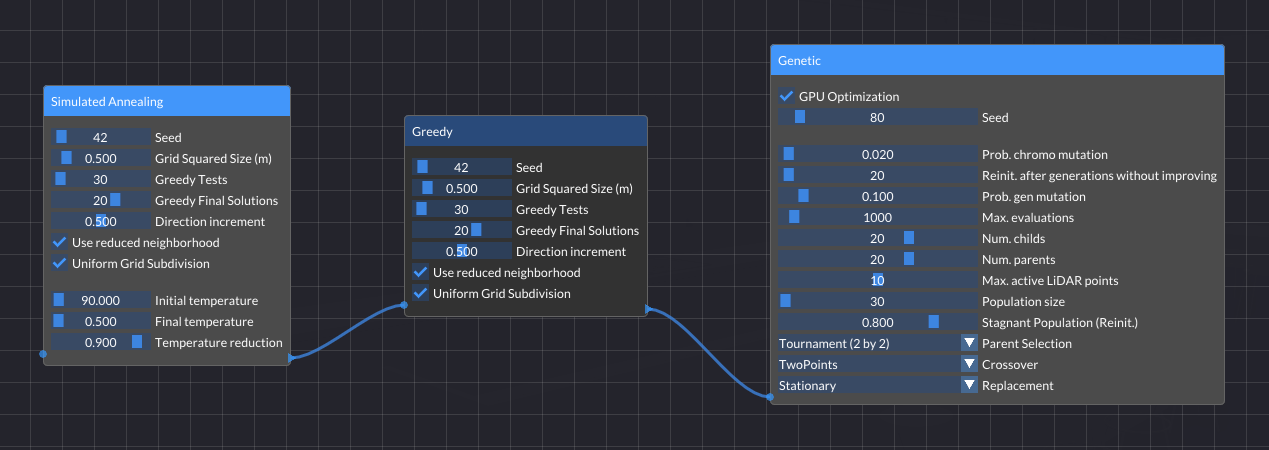
\includegraphics[width=\linewidth]{figs/lidar_optimization/optimization_node_editor.png}
	\caption{Three different environments authored by Autodesk Revit \textregistered \hspace{.5mm}. a) A basement with 130k triangles ($20 \times 4 \times 21$\si{\meter}), b) a school with 500K triangles ($44 \times 24 \times 32$\si{\meter}) and c), an office building with 2.7M triangles ($16 \times 8 \times 49$\si{\meter}). }
	\label{fig:optimization_node_editor}
\end{figure*}

\section{Results and discussion}

\begin{figure*}
    \centering
    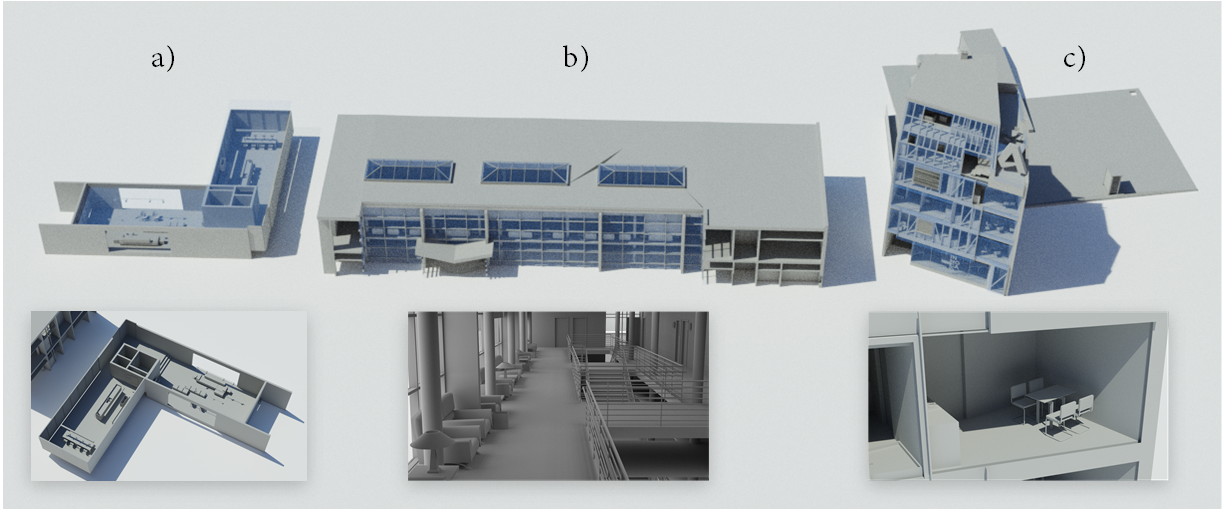
\includegraphics[width=\linewidth]{figs/lidar_optimization/evaluation_scenes.png}
	\caption{Three different environments authored by Autodesk Revit \textregistered \hspace{.5mm}. a) A basement with 130k triangles ($20 \times 4 \times 21$\si{\meter}), b) a school with 500K triangles ($44 \times 24 \times 32$\si{\meter}) and c), an office building with 2.7M triangles ($16 \times 8 \times 49$\si{\meter}). }
	\label{fig:bim_environments}
\end{figure*}

The proposed optimization has been tested against three different scenes from commercial software (see Figure \ref{fig:bim_environments}), exported as \verb|.obj| files and with a size ranging from 130K polygons to 2.7M. Although there exist a few studies concerning P4S in 3D, these solutions have not been openly published, and therefore, comparisons have been merely focused on the metrics performance and the speedup in comparison with a multi-core CPU-based approach. The latter version is implemented using OpenMP when possible; however, the LiDAR simulations are very time-consuming and both approaches solve them in the GPU. The configuration of local searches (LS from now on) is shown in Table \ref{table:local_search_settings}, whereas LiDAR specifications are detailed in Table \ref{table:optimization_lidar_parameters}. All measurements were performed on a PC with AMD Ryzen Threadripper 3970X 3.6 GHz, 256 GB RAM, two Nvidia RTX A6000 GPU and Windows 10 OS. 

\renewcommand{\arraystretch}{1.15}
\begin{table}[hb]
\caption{Configuration of parameters concerning greedy, simulated annealing and tabu search algorithms.}
\label{table:local_search_settings}
\begin{tabular}{@{}ll@{}}
\toprule
\textbf{Attributes} & \textbf{Value}\\
\midrule
Starting solutions & Grid sampling\\
Number of final solutions & Without restrictions\\
Voxel size & 0.5 \si{\meter} $\times\hspace{1mm}$0.4 \si{\meter}\\
\midrule
Max. number of iterations & 60\\
Max. number of iterations without improvements & 10\\
\midrule
Neighbourhood & Discrete (16)\\
Length of neighbourhood steps ($\Delta$) & 0.05 $\si{\meter}$\\
\midrule
Initial temperature ($T_0$) & 450$^{\circ}$C\\
Temperature decrease ($T_z$) & 0.8 $T_{z-1}$\\
\bottomrule
\end{tabular}
\end{table}
\renewcommand{\arraystretch}{1}

\renewcommand{\arraystretch}{1.15}
\begin{table}
\caption{Specifications of LiDAR sensor during optimization, following the commercial device HDL-64E. Attributes with * have }
\label{table:optimization_lidar_parameters}
\begin{tabular}{p{0.51\linewidth}p{0.4\linewidth}}
\toprule
\textbf{Attributes} & \textbf{Value}\\
\midrule
Resolution & 4500 $\times\hspace{1mm}$ 64 beams\\
Maximum number of returns & 1\footnote[1]{It has been adapted to reduce the optimization latency.}\\
Maximum range & 5\si{\meter}\footnote[2]{It has been adapted to improve the accuracy of the results.}\\
Coverage & 360\textdegree x 26.9\textdegree$\hspace{1mm}$(-24.9\textdegree-2\textdegree)\\
Height coverage & [0.5, 2] \hspace{.3mm}\si{\meter}\\
Minimum \textit{xz} distance to items & 0.4 \si{\meter}\\
Vertical tests & r $\gets$ 0.2 \si{\meter}, n $\gets$ 16 rays\\
%Interleaved solution distance & 4 \si{\meter}\\
\bottomrule
\end{tabular}
\end{table}
\renewcommand{\arraystretch}{1}

This section is organized as follows. First, the performance of different LS algorithms is evaluated regarding $F_1$ and $F_2$ metrics. Then, LS and GA algorithms are combined to seek the best pipeline, also in terms of metrics. CPU and GPU approaches are assessed according to the measured response time, and finally, we study which are the effects of varying the LiDAR height in the optimization.

\subsection{Performance of local searches}

This section shows how local searches improve the $F_2$ results using greedy, traditional LS, simulated annealing and tabu search algorithms. The basement scene is used during these tests, and the evaluation of $F_2$ for each initial solution is depicted regardless of the best solution observed until a specific iteration. Although LS reachs huge improvements, the relevance of applying the GA selection is evidenced by Figure \ref{fig:greedy_results}. It shows the narrowing phase of a greedy algorithm selecting the best $k \gets 30$ scans (red) in a scenario with areas that present different geometrical complexity, guided by the minimization of the $F_2$ metric. Hence, most of the selected locations are surrounded by dense geometry. Still, it manages to cover most of the scene. Similarly, small enclosed rooms, as the zoom-in of Figure \ref{fig:greedy_results}, are not scanned since their enclosed scans have a lower number of scanned polygons and thus worse metric values.

\begin{figure}
    \centering
    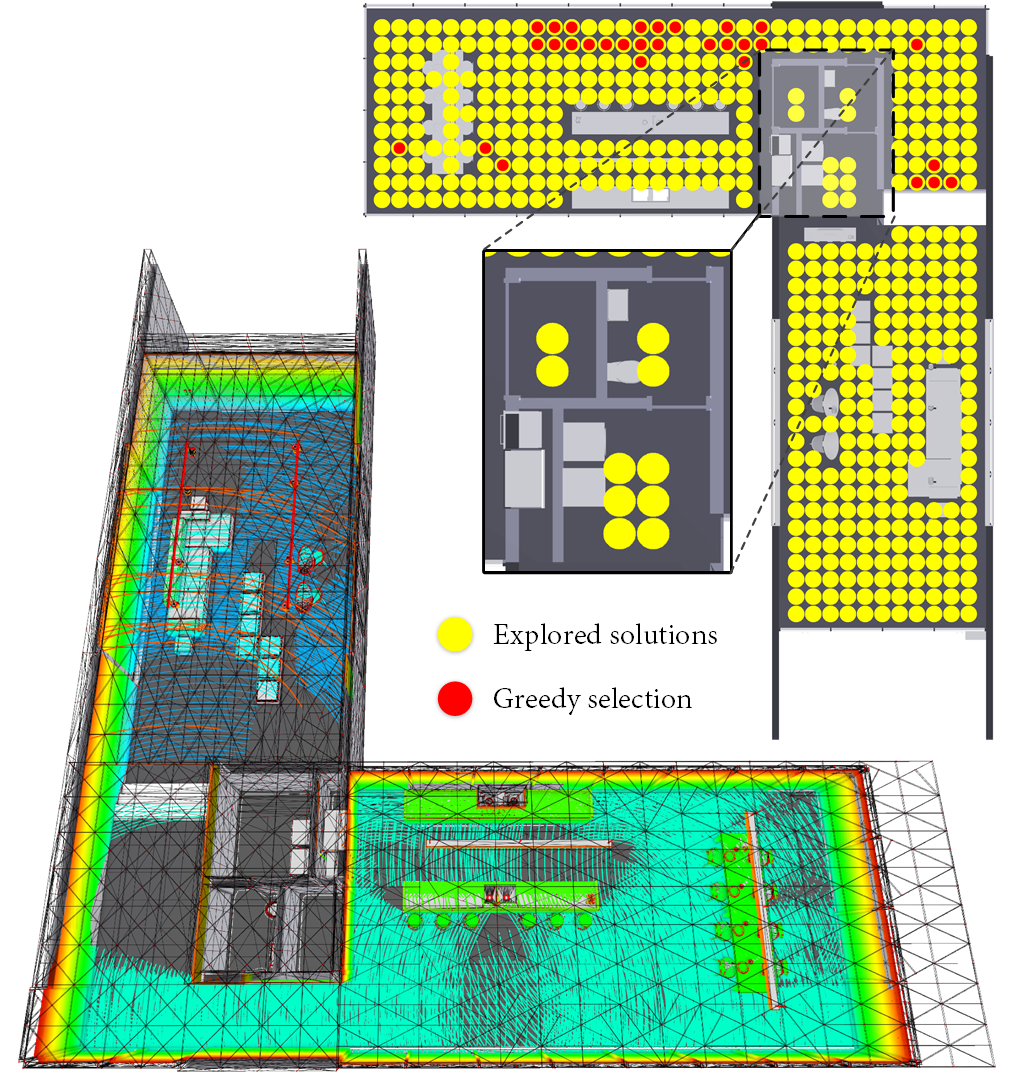
\includegraphics[width=\linewidth]{figs/lidar_optimization/greedy_results.png}
	\caption{Selection of the best thirty LiDAR scans with a greedy approach in the basement scene.}
	\label{fig:greedy_results}
\end{figure}

\begin{figure*}
    \centering
    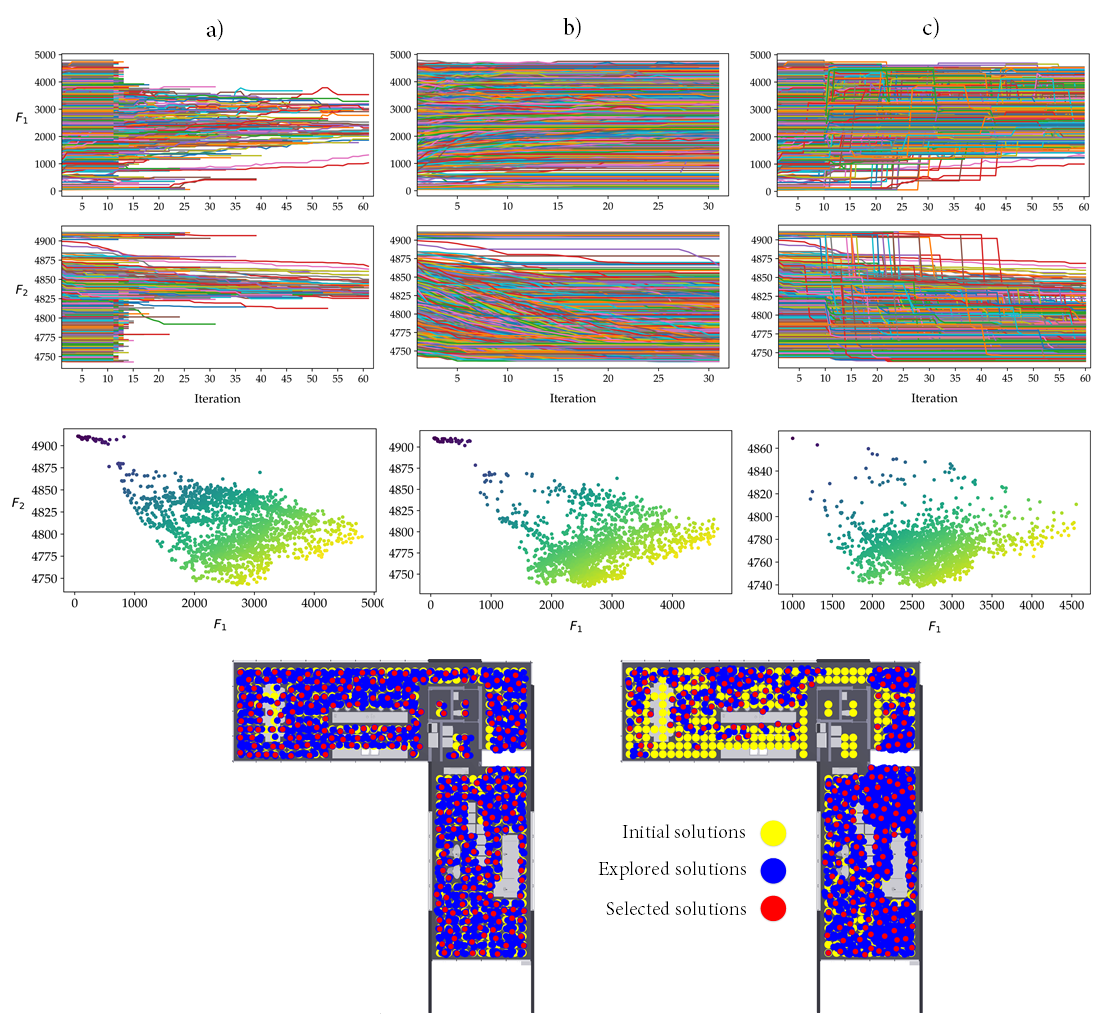
\includegraphics[width=.9\linewidth]{figs/lidar_optimization/local_search_results.png}
	\caption{Optimization obtained using a a) naive LS, b) SA and c) TS, showing both $F_1$ and $F_2$ results through a timeline and the final distribution. The bottom images show the locations optimized with SA and TS, organized into a regular grid and filtered by selecting only one solution per subdivision.}
	\label{fig:local_search_results}
\end{figure*}

From the greedy baseline, Figure \ref{fig:local_search_results} depicts the changes of initial solutions when different local searches are applied to them. For that purpose, $F_1$ and $F_2$ results from individual solutions are depicted during up to sixty iterations. However, some explorations, such as SA, were finished earlier since the temperature also converged earlier or no better solutions were found. Optimized locations are not narrowed using GA, and therefore, those depicted are filtered according to a regular grid that allows selecting a single solution per cell.

\textbf{Local search}. As expected from previous descriptions, the explorations of LS finish early, especially for locations that start with low $F_2$ values. The algorithm is not allowed to move to worse solutions, thus rapidly achieving the maximum number of iterations. Also, changes are controlled with a small factor; otherwise, the grid-like sampling would turn into a random sampling. Due to the naïve mechanism of LS, most locations converged into locations very close to walls, as regarded by \cite{soudarissanane_optimizing_2012}, since these maximize $F_1$ (number of collisions) with a low incidence angle (good accuracy).

\textbf{Simulated annealing}. As opposed to LS, SA is able to temporarily worsen the metric results and helps to explore a wider area in \textit{xz} and \textit{y}. Hence, most of the initial locations reached lower values of $F_2$ than LS, as shown in the scatter plot. Implicitly, initial solutions move to locations that cover a larger number of polygons since $F_1$ is also integrated into $F_2$ definition. However, early-finished explorations were not as frequent as in LS. Despite LOC being included in $F_2$, the line graph shows iterations that reached a lower number of collided polygons than previous solutions, i.e., worsened the LOC metric. It is not correlated to SA accepting worse solutions, since LOC is not a primary metric at this stage; instead, it is the consequence of changes that improve their accuracy at expense of worsening the coverage. For that reason, the subsequent GA stage is mainly guided by the LOC metric.

\textbf{Tabu search}. Avoiding previous moves and re-initializing when getting stuck seems to make final solutions more optimal in terms of $F_2$ (not for $F_1$) than those obtained by previous algorithms. However, improved locations were not uniformly sparsed as they 1) tend to show a preference for areas with higher geometrical density and 2) random re-initialization favours this. Despite this being desirable, the local improvement of SA is preferred over TS as it offers a wider range of possibilities to the later GA, whereas TS offers immediate results. Also, note that the steeper metric signatures are the result of re-initialization since it involves selecting a new set of random points. Without re-initialization, TS turns into a more strict LS.

\subsection{Pipeline performance}

\begin{figure*}
    \centering
    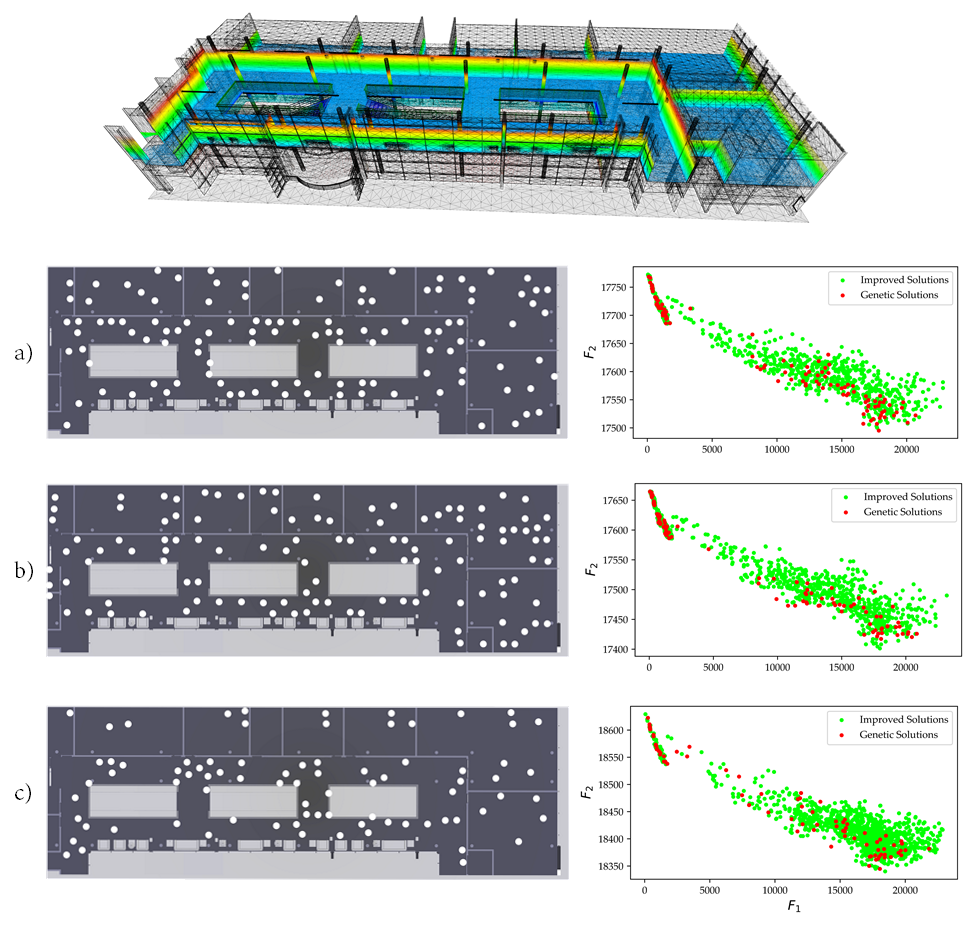
\includegraphics[width=.85\linewidth]{figs/lidar_optimization/ga_results.png}
	\caption{Results of combining local searches and genetic algorithms. The left images depict the final LiDAR distribution, whereas the right images show the improvement of intermediate results with regard to the proposed metric ($\textit{Y} \gets$ Minimization, $\textit{X} \gets$ Maximization). a), b) and c) refer to LS + GA, SA + GA and TS + GA combinations. }
	\label{fig:genetic_results}
\end{figure*}

One of the main challenges of planning LiDAR set-ups is to cover the whole building level, including enclosed rooms. However, previous approaches optimize local metrics, whereas the sorting and narrowing of locations according to $F_2$ only guarantee that selected locations provide dense coverage of \textbf{their} area. A better selection is expected to be provided by GAS guided by a global metric measuring the polygon coverage. The evaluated GA was launched using the configuration in Table \ref{table:genetic_algorithm_parameters}. Also, GAs do not operate alone, but they are supported by a starting LS. Hence, different combinations are checked, including LS + GA, SA + GA and TS + GA. Besides coverage, the intrinsic selection of LiDAR locations is also observed during these tests.

The results for three different pipelines are depicted in Figure \ref{fig:genetic_results}, using a single level of the school building. This scenario includes multiple enclosed rooms that cannot be scanned from central areas, as well as gaps in the central area that lead to scanning lower building levels. In this regard, the tabu search (c) obtained a lower number of points, though most of them are gathered in the main room, similar to locally improved solutions being translated to areas with higher geometrical complexity. In contrast to the tabu search, LS and SA provided a higher variety of locations, thereby helping to select a higher number of locations that provide better coverage of enclosed rooms. Also, note that the LiDAR range was limited to $r \gets 5 \si{\meter}$ to account for the accuracy loss, and therefore, higher values of $r$ inevitably obtain a smaller selection. Despite LS and SA providing similar results, the pipeline SA + GA managed to scan the small rooms on the left and right sides due to its wider exploration. Nevertheless, the performance in terms of $F_1$ and $F_2$ was similar for every spatial search, as shown in the scatter plots. It can be concluded that the spatial search preceding the GA has a relevant weight in the final output.

\renewcommand{\arraystretch}{1.15}
\begin{table}
\caption{Parameters of the genetic algorithm launched in this stage.}
\label{table:genetic_algorithm_parameters}
\begin{tabular}{ll}
\toprule
\textbf{Attributes} & \textbf{Value}\\
\midrule
Maximum number of evaluations & 50.000\\
Population size & 500\\
Number of parents & 250\\
$\mathcal{P}$(Chromosome mutation) & 0.02\\
$\mathcal{P}$(Gen mutation) & 0.1\\
Stagnant population (re-initialization) & 80\%\\
Stuck at local minima (re-initialization) & 30 it. without improving\\
Crossover operator & Two points\\
Selection operator & 2-tuple tournament\\
Kind of replacement & Stationary\\
\bottomrule
\end{tabular}
\end{table}
\renewcommand{\arraystretch}{1}

\subsection{Level of overlap}

Previous LiDAR locations were improved and selected according to $F_1$ and $F_2$ metrics to fit the LOC, LOD and LOA requirements. However, LOO was not considered during these optimizations. Instead, it is considered after GA selection by including new locations aimed at improving the overlapping rather than providing an optimal solution. In this section, we carry out some tests about LOO using a greedy approach to 1) sample the scenario and 2) narrow it to a few solutions scattered by controlling the spatial density. Accordingly, Figure \ref{fig:loo_results} shows the initial overlapping as well as the improvement after requiring an overlap of 20\%, 40\% and 60\%. Below, the LiDAR locations are obtained by limiting the sensor range to 1.5 \si{\meter} and 1 \si{\meter}, respectively. Initial solutions were not improved by means of local searches, thus displaying a grid-like pattern. The last test shows an experiment where the overlapping challenge was further pushed by scattering solutions with a minimum distance of (6 - $\epsilon$) \si{\meter}. Therefore, the minimum number of solutions to reach one another is 2, though it varies according to their distance. 

\begin{figure}
    \centering
    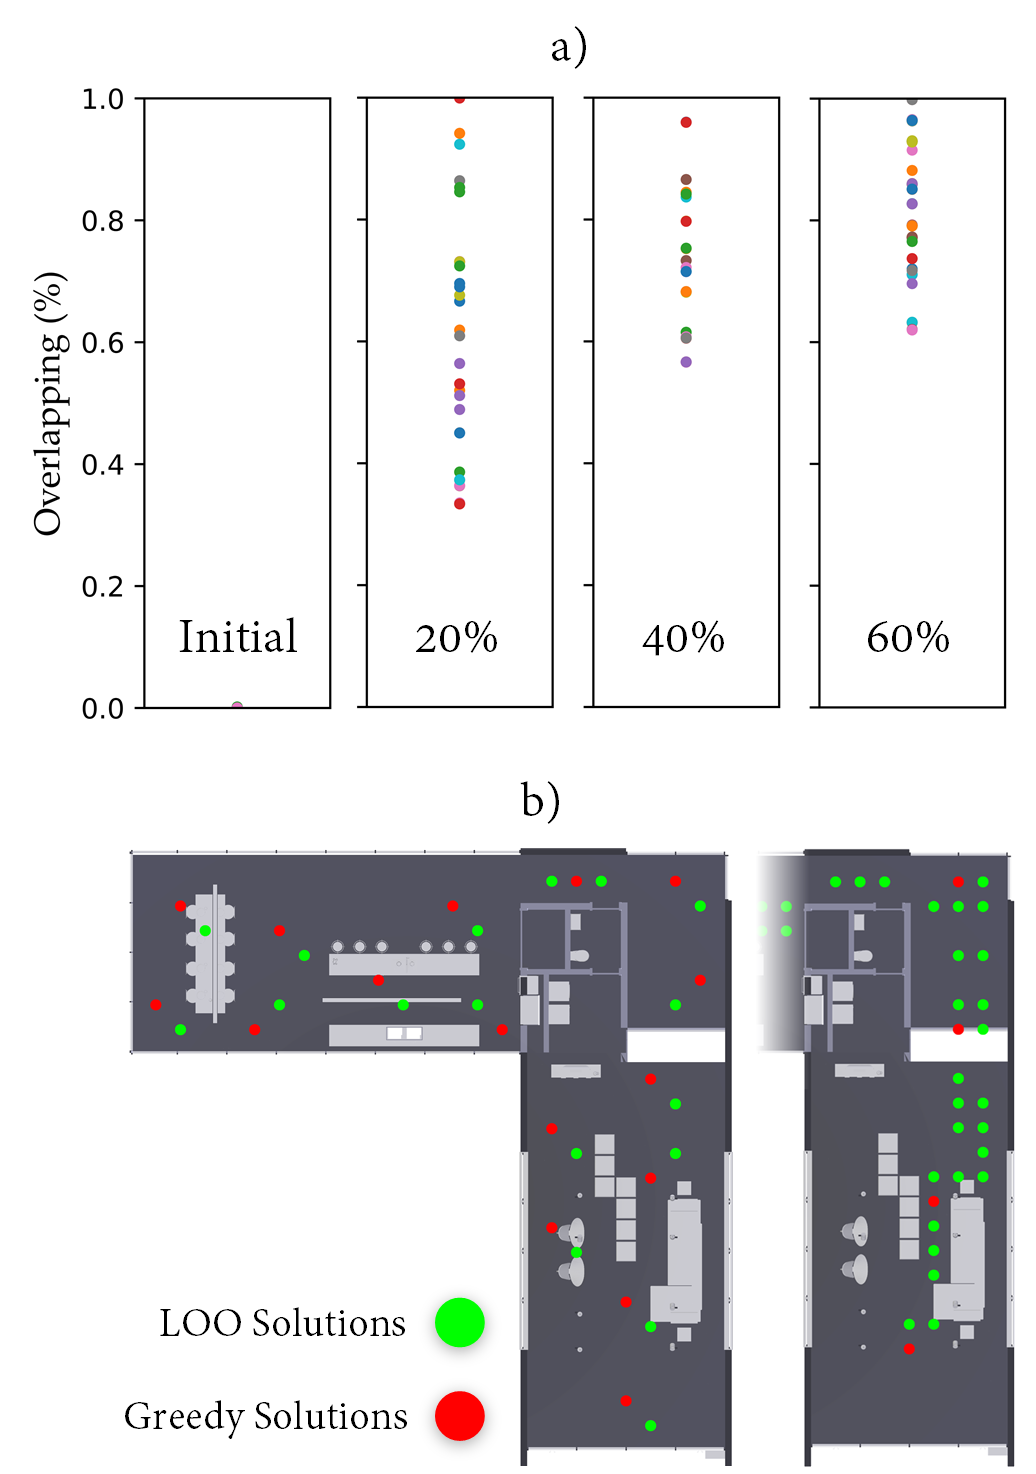
\includegraphics[width=\linewidth]{figs/lidar_optimization/loo_results.png}
	\caption{a) Initial overlap and the results obtained after requiring an overlap of 20\%, 40\% and 60\%. b) Rendering of LiDAR scans selected by a Greedy approach as well as those selected by the proposed method to enhance the overlap. }
	\label{fig:loo_results}
\end{figure}

\subsection{Response time}

The main drawback of these optimization algorithms is that they require solving LiDAR scans sequentially. The spatial searches cannot be solved in parallel, whereas the GA algorithm can be massively parallelized by 1) solving the whole LiDAR simulation of a chromosome at once, since it is composed of several locations, and 2) evaluating large populations. A more efficient approach is to make pre-calculations at expense of a higher CPU memory footprint. Hence, some optimizations and implementation details are here discussed to provide the most efficient solution available.

Current LS-based algorithms check the validity of every new solution, and estimate the metric values, regardless of the fact that it could have been previously checked. It seldom happens for randomized initializations, but it is very frequent in grid-like initializations with a constant step length. Therefore, it is possible to make this more efficient by calculating the validity and fitness of every voxel once, and using this during the optimization. To this end, voxels must have a size equivalent to the step length. The baseline response time is given by the greedy approach, which is not affected by the proposed acceleration techniques. Figure \ref{fig:local_search_response_time} shows the average and global response time for LS, SA and TS algorithms. Tests were conducted over the office building using the configuration in Table \ref{table:local_search_settings}: the first chart shows the response time per evaluated location, whereas the chart on the right side shows the overall response time. From these results, it can be observed that latency varies depending on the LiDAR location and how hard was to traverse the BVH from that position. From the summed results it can be inferred that this pre-calculation approach significantly speed-ups the procedure, with it being significantly larger as the number of iterations increase and processes do not terminate.

\begin{figure*}
    \centering
    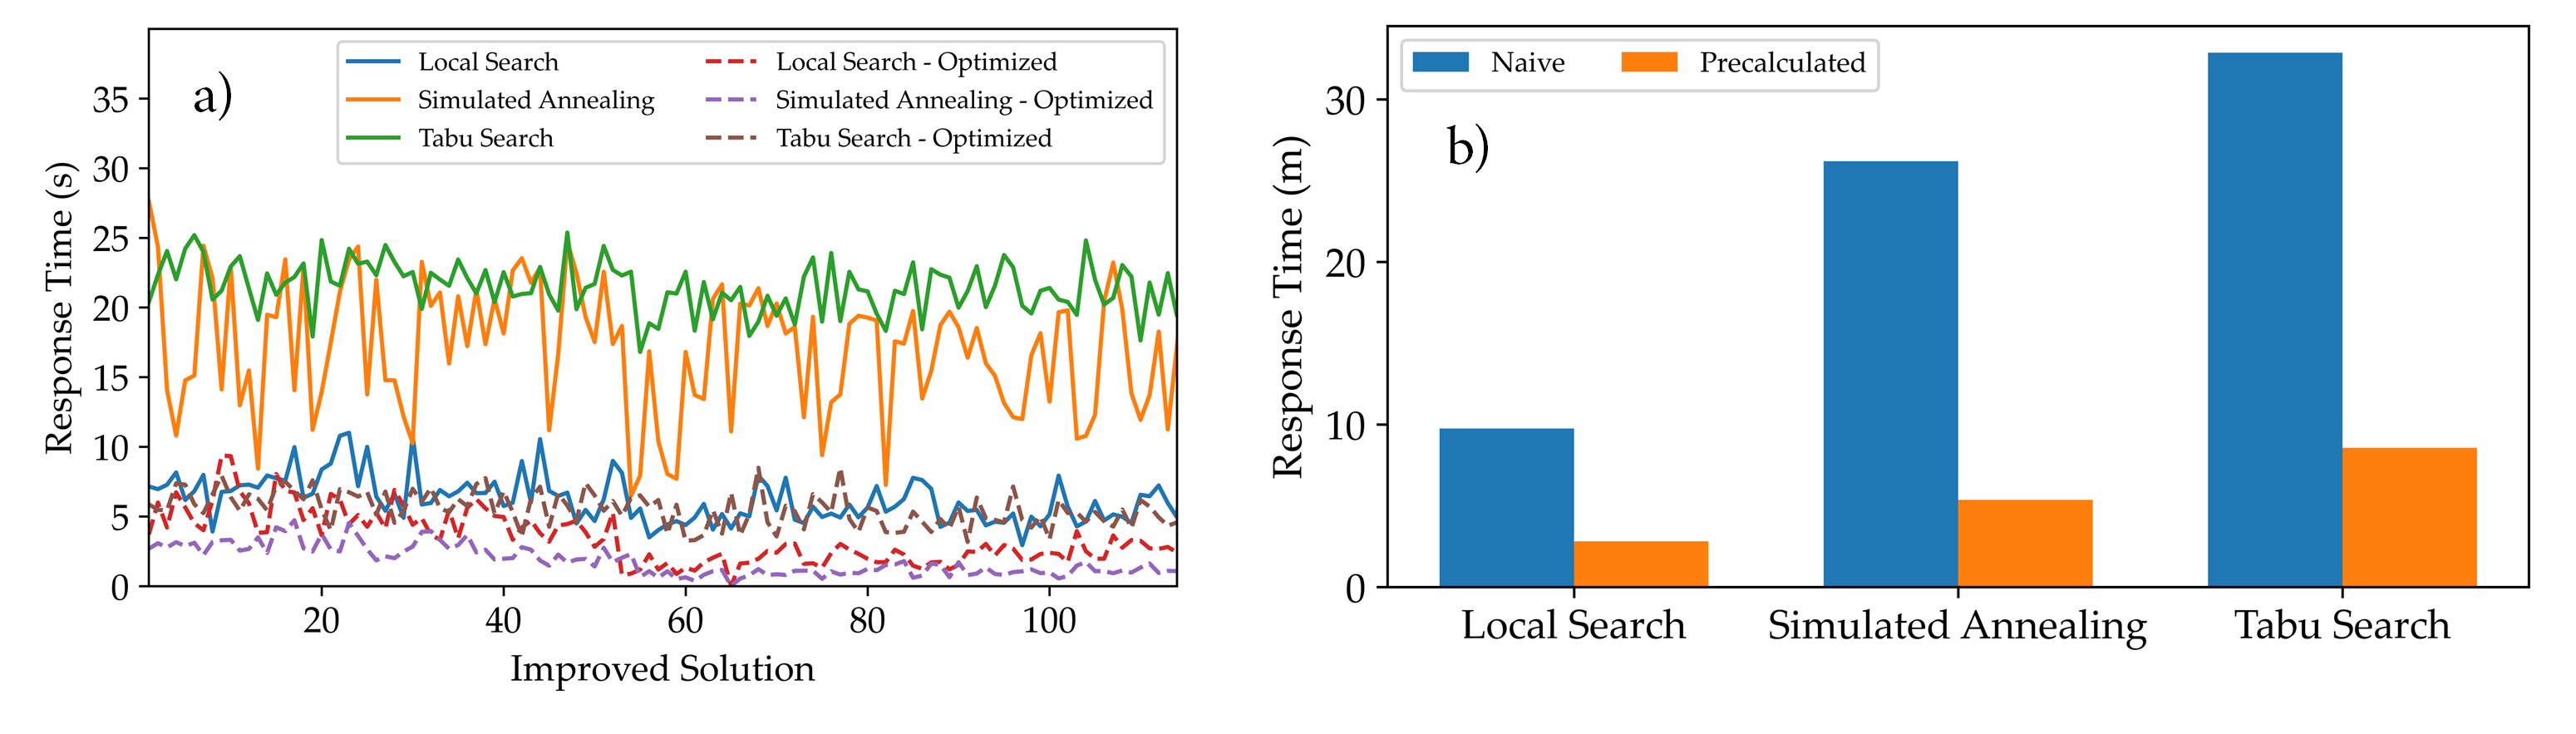
\includegraphics[width=.9\linewidth]{figs/lidar_optimization/response_time_results.png}
	\caption{a) The average response time per scan for LS algorithms, implemented by following two approaches: naïve and optimized, and b) summation of response time from previous configurations.  }
	\label{fig:local_search_response_time}
\end{figure*}

During the selection stage, different chromosomes are evaluated synchronously. Parallelism is present in other stages: initialization, parent selection, crossover, etc. Hence, we evaluated whether it was effective to implement the genetic algorithm pipeline on the GPU. Initially, it is implemented as a multi-thread solution on the CPU. From Figure \ref{fig:local_search_response_time} we can observe that the GPU-based solution is significantly faster. It mainly occurs due to data being processed in the GPU for the whole GA pipeline, instead of transferring it before and after evaluating the solution's fitness (see Figure \ref{fig:ga_response_time}).

\begin{figure}
    \centering
    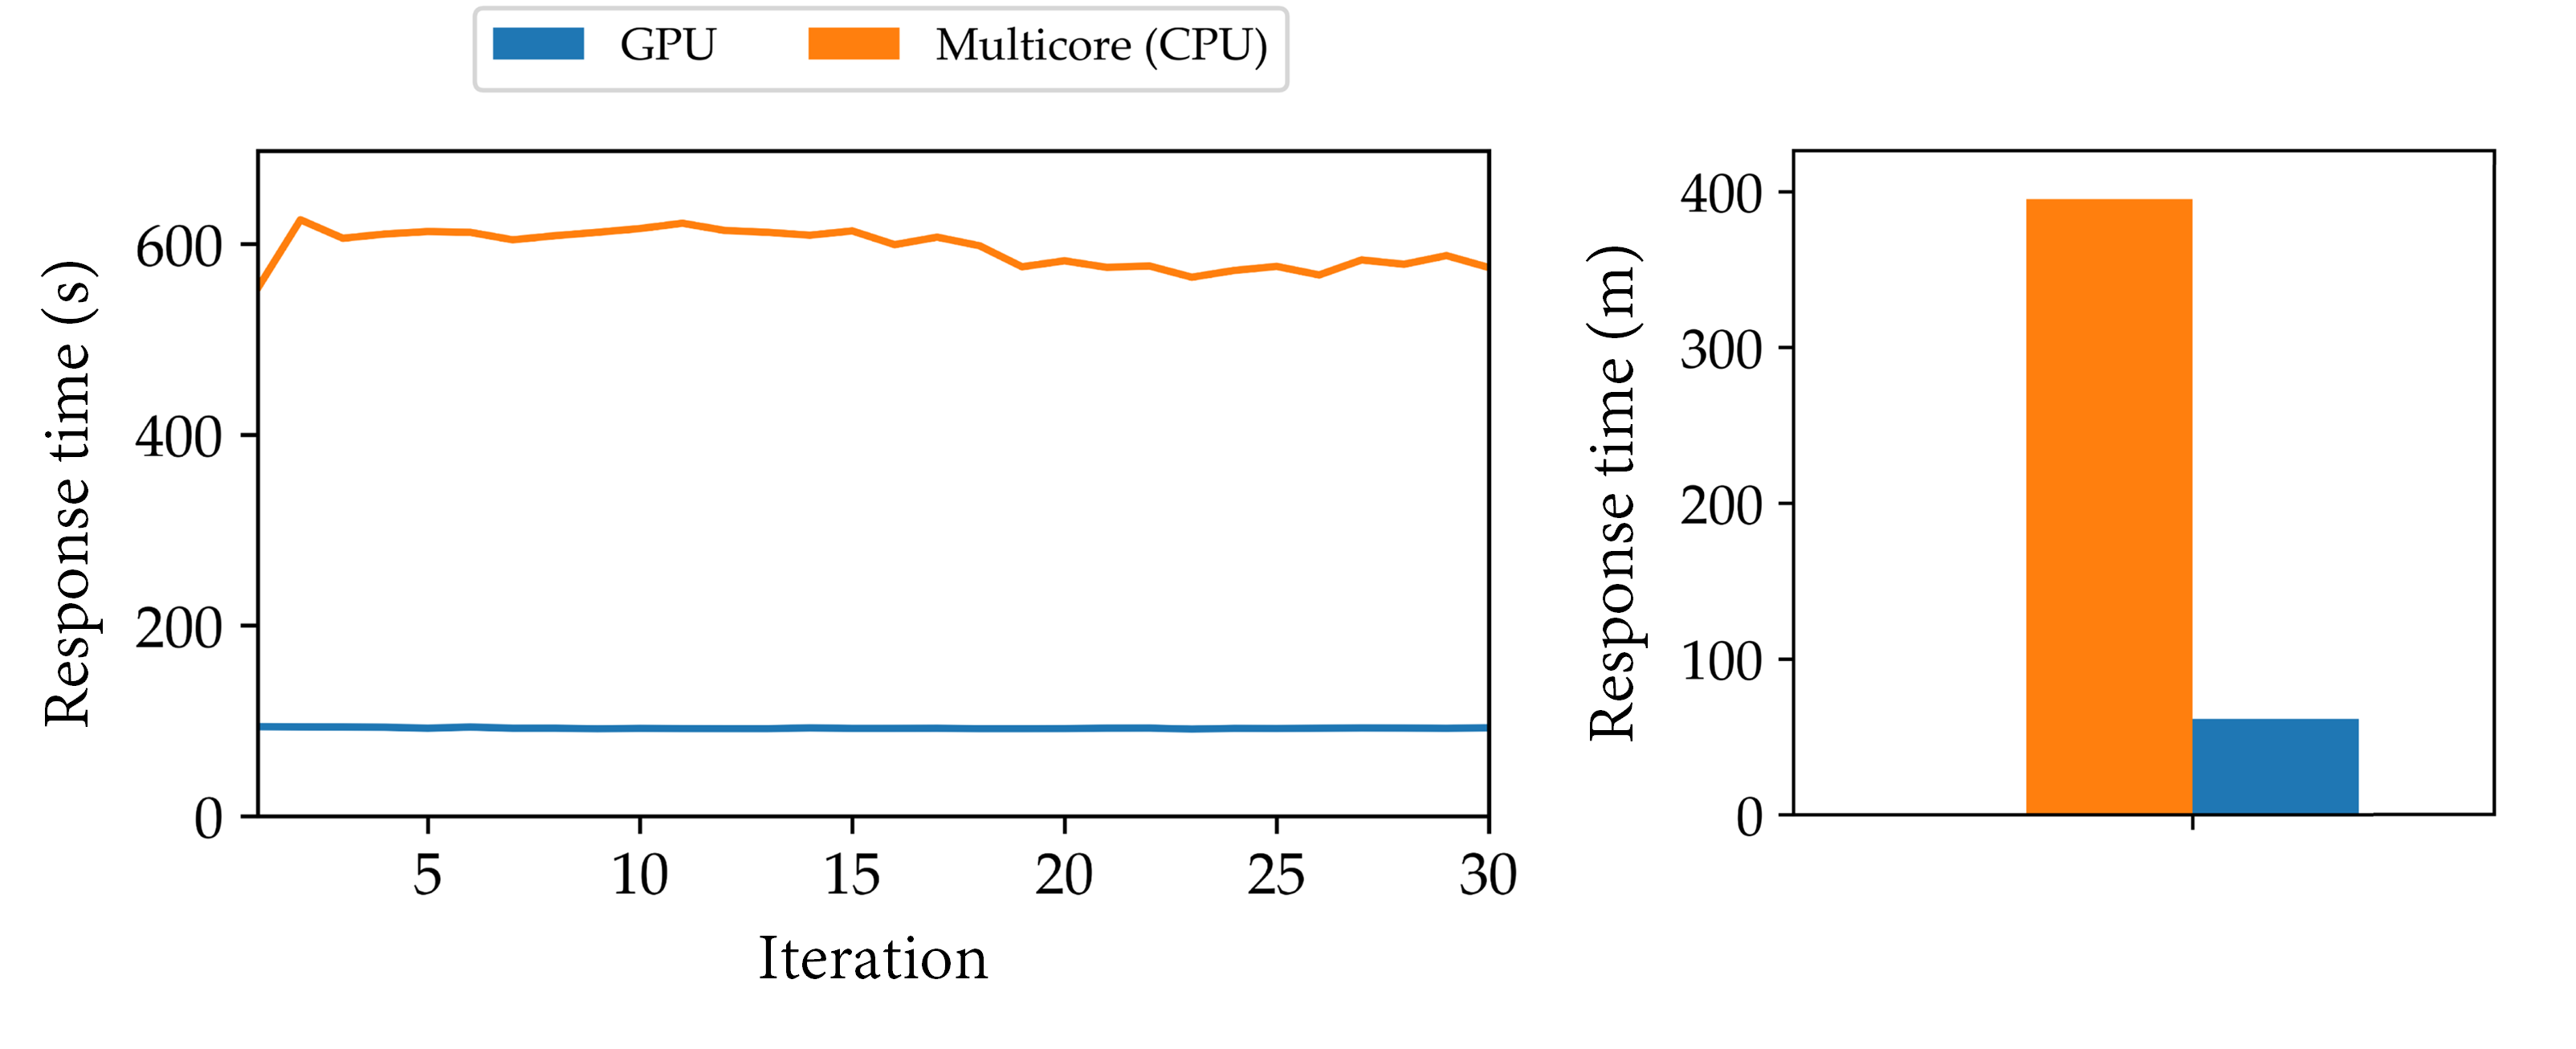
\includegraphics[width=.6\linewidth]{figs/lidar_optimization/response_time_results_ga.png}
	\caption{Response time of genetic algorithms implemented as CPU (multi-core) and GPU solutions. First, the response time is shown per GA population, and finally, the response time is summed for each sort of optimization.}
	\label{fig:ga_response_time}
\end{figure}

\subsection{Variable scan height}

Another contribution of this work is the estimation of the most appropriate scanning height. Figure \ref{fig:cubicle_room} shows the results of $F_1$ and $F_2$ metrics by using 1) fixed height or 2) variable height within the range (1 \si{\meter}, 2 \si{\meter}). In both cases, the scenario is uniformly subsampled every 0.1 \si{\meter}. Accordingly, the first search is performed over a 2D grid, regardless of being applied over a 3D scene, whereas the second one is 3D. The results are obtained using a test environment composed of four outer walls and four inner walls, where the latter has each one a gap at a different height, as depicted in Figure \ref{fig:cubicle_room}. The LiDAR was first configured as a Velodyne HDL-64E, and then, as a Pandar64 with a wider vertical Field of View (FOV) and non-uniform resolution. Instead of LS, a Greedy approach was used to evaluate a fine-grained subdivision of the space that is subsequently narrowed to the top-ten locations. As observed in Figure \ref{fig:cubicle_room}, the scans selected by the Greedy approach are placed next to wall holes, thereby allowing to reach more polygons despite being guided by the $F_2$ metric. Therefore, this shows the inclusion of $F_1$ in $F_2$ as well as the capabilities of the proposed pipeline to adapt to different optimal heights..

\begin{figure*}
    \centering
    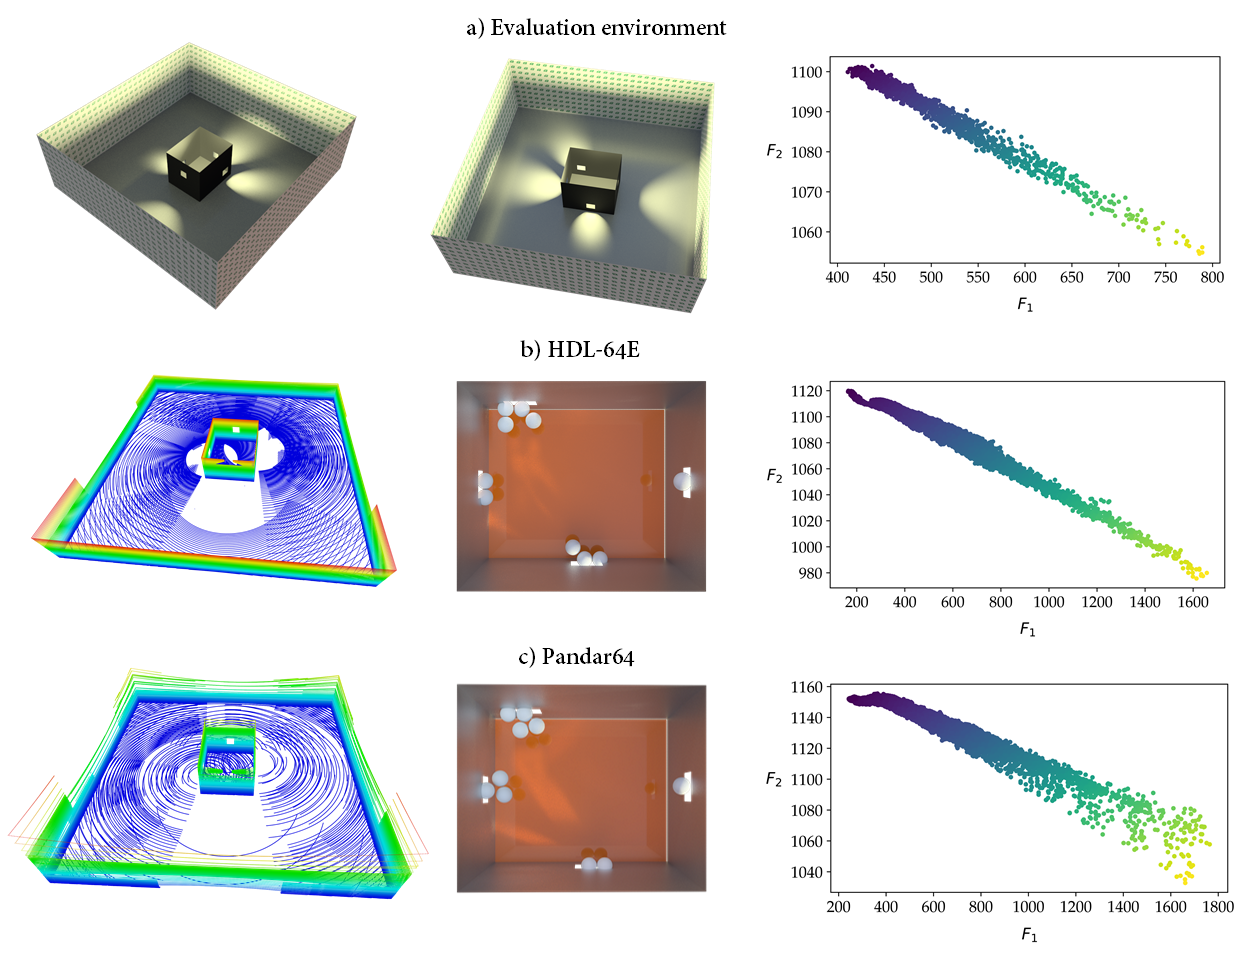
\includegraphics[width=\linewidth]{figs/lidar_optimization/height_variability.png}
	\caption{a) An environment designed for testing the benefits of variable height, and b, c) locations selected by a Greedy algorithm using HDL-64E and Pandar64 LiDAR sensors. The scatter plots show the values of $F_1$ and $F_2$ for each initial solution. The first one shows the results of a LiDAR with a fixed height. }
	\label{fig:cubicle_room}
\end{figure*}

\section{Conclusions and future work}

A planning for scanning methodology was described to select the best locations in 3D environments. These were not simplified nor reduced to cross-sections, and parameters derived from the scenario, such as the resolution, were automatically estimated. Part of the objective function, which includes a LiDAR simulation, was solved in the GPU. Instead of using a single metaheuristic, several were proposed to be chained to exploit exhaustivity (genetic algorithms) and exploration (spatial search) taking advantage of GPU-based spatial queries and LiDAR scans. Four objective functions were formulated without relying on user-defined parameters or thresholds. Among them, $F_2$ metric was further improved to account for $F_1$ and a traditional $F_2$ metric. Also, the optimal number of scans is intrinsically discovered by a genetic algorithm, instead of being configured. The results show that this pipeline is capable of achieving a nearly optimal network of LiDAR scans that can be later fused while densely and accurately covering the scenario. 

As future work, we would like to reduce the latency, which is still time-consuming due to the large input scenarios and LiDAR simulations, despite being accelerated in the GPU. Pre-calculating ought to be further explored, at expense of memory footprint. In this regard, compression may be a key factor due to the similarity of spatially close scans. Finally, this optimization approach could be extended to other kinds of LiDAR, including those that require a path rather than a set of discrete locations (e.g., mobile and aerial LiDAR). 
